% ****** Start of file apssamp.tex ******
%DIF LATEXDIFF DIFFERENCE FILE
%DIF DEL Xu_Avila_PRL19_orig.tex   Tue Aug 27 10:44:03 2019
%DIF ADD Xu_Avila_PRL19.tex        Tue Aug 27 10:44:03 2019
%
%   This file is part of the APS files in the REVTeX 4.2 distribution.
%   Version 4.2a of REVTeX, December 2014
%
%   Copyright (c) 2014 The American Physical Society.
%
%   See the REVTeX 4 README file for restrictions and more information.
%
% TeX'ing this file requires that you have AMS-LaTeX 2.0 installed
% as well as the rest of the prerequisites for REVTeX 4.2
%
% See the REVTeX 4 README file
% It also requires running BibTeX. The commands are as follows:
%
%  1)  latex apssamp.tex
%  2)  bibtex apssamp
%  3)  latex apssamp.tex
%  4)  latex apssamp.tex
%
\documentclass[aps,prl,reprint,superscriptaddress,floatfix]{revtex4-1}


\usepackage{graphicx}% Include figure files
%\usepackage{dcolumn}% Align table columns on decimal point
%\usepackage{bm}% bold math
%\usepackage{epstopdf, epsfig}
\usepackage{amsmath}
\usepackage{amssymb}
%\usepackage{mathtools}
%\usepackage{hyperref}
%\usepackage{booktabs} % To thicken table lines


\newcommand{\Rey}{\mathit{Re}}
\newcommand{\Wo}{\mathit{Wo}}
\newcommand{\A}{\mathit{A}}
\renewcommand{\H}{\mathit{H}}% Reynolds number
%DIF PREAMBLE EXTENSION ADDED BY LATEXDIFF
%DIF UNDERLINE PREAMBLE %DIF PREAMBLE
\RequirePackage[normalem]{ulem} %DIF PREAMBLE
\RequirePackage{color}\definecolor{RED}{rgb}{1,0,0}\definecolor{BLUE}{rgb}{0,0,1} %DIF PREAMBLE
\providecommand{\DIFadd}[1]{{\protect\color{blue}\uwave{#1}}} %DIF PREAMBLE
\providecommand{\DIFdel}[1]{{\protect\color{red}\sout{#1}}}                      %DIF PREAMBLE
%DIF SAFE PREAMBLE %DIF PREAMBLE
\providecommand{\DIFaddbegin}{} %DIF PREAMBLE
\providecommand{\DIFaddend}{} %DIF PREAMBLE
\providecommand{\DIFdelbegin}{} %DIF PREAMBLE
\providecommand{\DIFdelend}{} %DIF PREAMBLE
%DIF FLOATSAFE PREAMBLE %DIF PREAMBLE
\providecommand{\DIFaddFL}[1]{\DIFadd{#1}} %DIF PREAMBLE
\providecommand{\DIFdelFL}[1]{\DIFdel{#1}} %DIF PREAMBLE
\providecommand{\DIFaddbeginFL}{} %DIF PREAMBLE
\providecommand{\DIFaddendFL}{} %DIF PREAMBLE
\providecommand{\DIFdelbeginFL}{} %DIF PREAMBLE
\providecommand{\DIFdelendFL}{} %DIF PREAMBLE
%DIF END PREAMBLE EXTENSION ADDED BY LATEXDIFF

\begin{document}

\preprint{}

\title{Resonances in pulsatile channel flow with an elastic wall}% Force line breaks with \\
%\thanks{A footnote to the article title}%

\author{Duo Xu}
 \email{duo.xu@zarm.uni-bremen.de}
\affiliation{University of Bremen, Center of Applied Space Technology and Microgravity (ZARM), 28359 Bremen, Germany}
\affiliation{Friedrich-Alexander-Universit{\"a}t Erlangen-N{\"u}rnberg, 91058 Erlangen, Germany}%
%
%\collaboration{MUSO Collaboration}%\noaffiliation

\author{Thomas Seeb{\"o}ck}
% \homepage{http://www.Second.institution.edu/~Charlie.Author}
\affiliation{Friedrich-Alexander-Universit{\"a}t Erlangen-N{\"u}rnberg, 91058 Erlangen, Germany}

\author{Marc Avila}
\email{marc.avila@zarm.uni-bremen.de}
\affiliation{University of Bremen, Center of Applied Space Technology and Microgravity (ZARM), 28359 Bremen, Germany}
\affiliation{Friedrich-Alexander-Universit{\"a}t Erlangen-N{\"u}rnberg, 91058 Erlangen, Germany}%

%\collaboration{CLEO Collaboration}%\noaffiliation

\date{\today}% It is always \today, today,
             %  but any date may be explicitly specified

\begin{abstract}
The interaction between fluid and elastic solids is ubiquitous in aerospace, mechanical and civil engineering. Pulsations in fluid velocity may interact with the natural frequency of the solids and lead to catastrophic events, such as the crumbling of the Tacoma-Narrows bridge. In nature, fluid-structure interaction is exploited by microorganisms to swim and it enables a reduction of the pressure and flow-rate pulsations of blood as this is transported from the heart to the periphery of the body.  Here we simplify this complex problem and consider the dynamics of a membrane clamped between two rigid segments in a channel. Fluid flow driven by a pulsatile pressure difference and after initial transients determined by the viscosity of the fluid, the membrane pulsates synchronously with the driving frequency. The amplitude of the oscillation varies non-monotonously with the governing parameters and exhibits strong resonances. At the resonance point, the flow rate over a cycle is larger than for steady flow in a rigid channel with the same pressure loss. We show that the oscillation motions of the elastic membrane can be accurately modeled with the equation of a forced damped harmonic oscillator. All key features of the system are predicted by the model: oscillation amplitude, phase between pressure driving and response of the membrane, resonance point and vanishing of the resonance as the viscous drag becomes dominant. 
\end{abstract}

%\keywords{Suggested keywords}%Use showkeys class option if keyword
                              %display desired
\maketitle

\DIFaddbegin \section*{\DIFadd{To Do}}
 \begin{itemize} 
\item \DIFadd{Check dim/non-dim quantities: Suggestion: Use uppercase for
  dimensional and lowercase for non-dimensional (only where a distinction
  is required!). You've already done
  this for the external pressure but I don't think it's totally
  consistent, but I may have screwed things up. Leave for now.
}\item \DIFadd{Make spelling (US/UK) consistent.
} \end{itemize} 

\DIFaddend Fluid flows through elastic conduits are of engineering and
physiological relevance. Locally in the arterial tree,
fluid-structure-interaction (FSI) can be harmful and has been
associated with the rupture of aneurysms~\cite{Han13} and
atherosclerotic plaque rupture in arterial stenoses, which can cause
heart attack or stroke \cite{Ku97}. On the other hand, in collapsed
blood vessels FSI is exploited to regulate the blood supply to
internal organs~\cite{Shapiro77}, and to help returning blood to the
heart during diastole~\cite{Casey08}. The fundamental setup to
investigate the nonlinearly coupled dynamics of the fluid and the
vessels is the Starling resistor~\cite{Knowlton12}, which consists of
an elastic tube mounted between two rigid tubes in a pressure
chamber. In the Starling resistor the fluid is driven at a steady flow
rate, but if the flow rate exceeds a critical value, self-excited
oscillations arise spontaneously~\cite{Bertram08,Heil10,Stewart09}. A
widely used system exhibiting similar dynamics is collapsible channel
flow, where fluid is driven between a rigid bottom wall and an upper
wall composed of a flexible externally pressurized membrane clamped
between two rigid  sections~\cite{Jensen03,Heil11}.
\DIFdelbegin \DIFdel{To the best of our knowledge, the fully coupled nonlinear interaction between pulsatile flow and an elastic wall has neither been investigated in channels nor in tubes.
}\DIFdelend \DIFaddbegin 

{\bf \DIFadd{*** there are forced studies; at least experimentally ***}}

\hrule

{\bf \DIFadd{*** STARTED HERE; STUFF ABOVE NOT TOUCHED YET ***}}

%DIF > To the best of our knowledge, the fully coupled nonlinear interaction
%DIF > between pulsatile flow and an elastic wall has neither been
%DIF > investigated in channels nor in tubes.

\DIFaddend \begin{figure}
	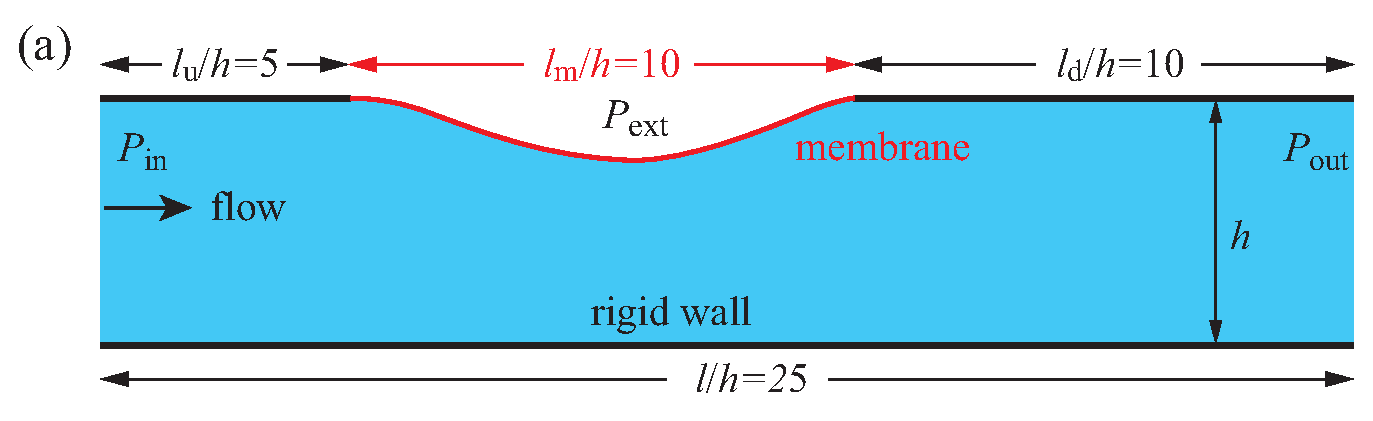
\includegraphics[width=1\linewidth, trim={0cm 0cm -0.35cm 0cm}, clip]{./epsFig/fig1a.eps}
	\DIFdelbeginFL %DIFDELCMD < 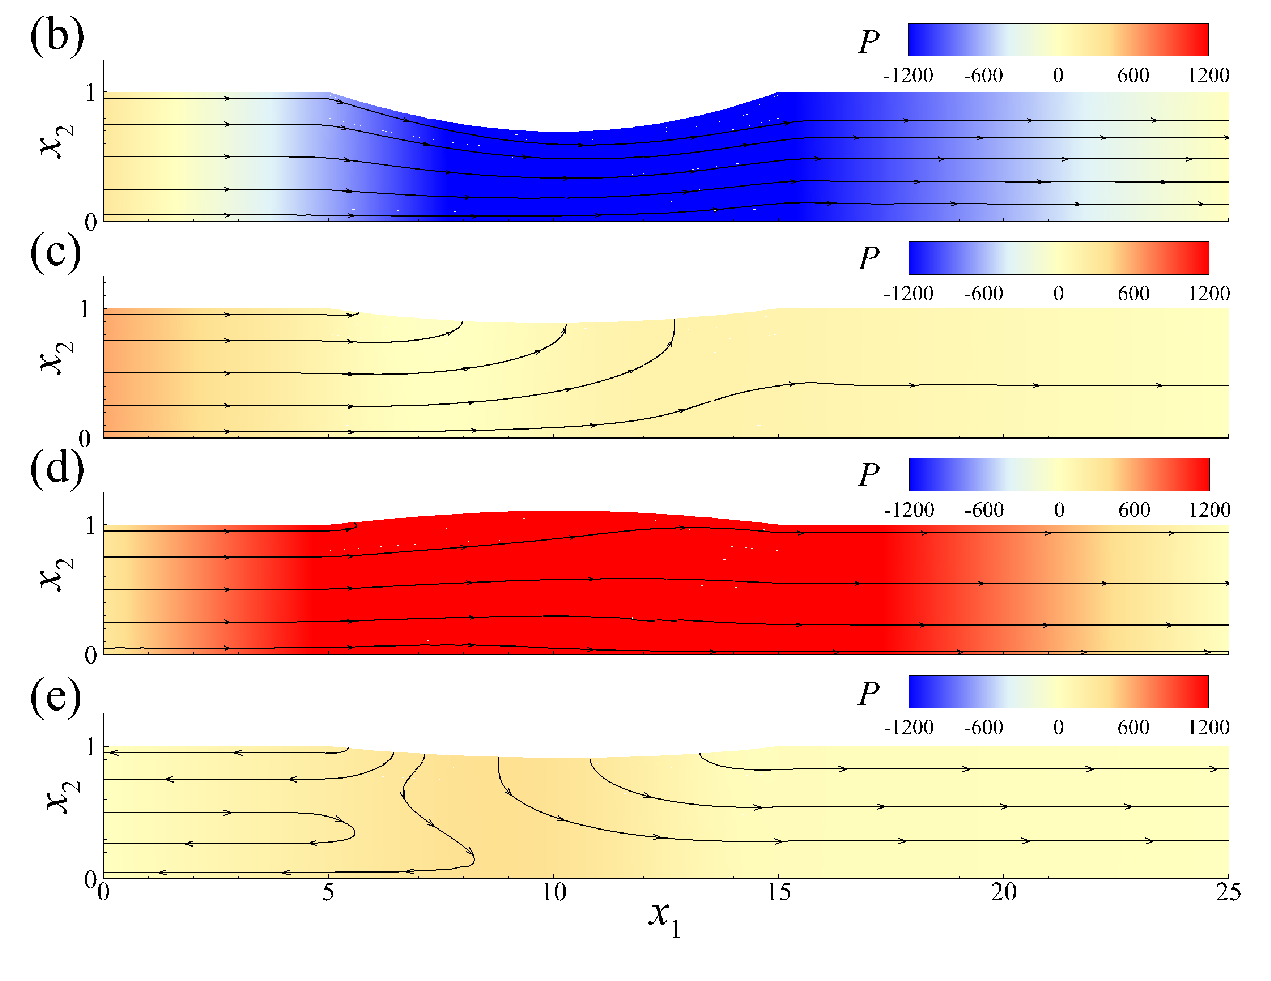
\includegraphics[width=1\linewidth, trim={0.2cm 0cm 0cm 0cm}, clip]{./epsFig/fig1b.eps}	
%DIFDELCMD < 	%%%
\DIFdelendFL \caption{\label{fig:setup}(Color online) \DIFdelbeginFL \DIFdelFL{(a) }\DIFdelendFL Sketch of fluid
          flow in a collapsible channel with an externally pressurized
          membrane clamped between two rigid walls. The flow is driven
          by a pulsatile pressure \DIFdelbeginFL \DIFdelFL{difference. Contour of pressure after }\DIFdelendFL \DIFaddbeginFL \DIFaddFL{applied at }\DIFaddendFL the \DIFdelbeginFL \DIFdelFL{initial transients for $t/T = 0$ (b), $0.25$ (c), $0.5$ (d) and $0.75$ }\DIFdelendFL \DIFaddbeginFL \DIFaddFL{upstream end.
          }{\bf \DIFaddFL{Kill label ``}\DIFaddendFL (\DIFdelbeginFL \DIFdelFL{e}\DIFdelendFL \DIFaddbeginFL \DIFaddFL{a}\DIFaddendFL )\DIFdelbeginFL \DIFdelFL{, and streamlines are marked in solid lines with arrows.}\DIFdelendFL \DIFaddbeginFL \DIFaddFL{'' ***}}
          {\bf \DIFaddFL{*** Change channel width to $a$ ***}}
          {\bf \DIFaddFL{*** State $p=0$ at outlet ***; *** Add
           coordinates to sketch ***}}\DIFaddendFL }
\end{figure}

In this \emph{Letter}, we perform numerical simulations of a
collapsible channel \DIFdelbegin \DIFdel{with }\DIFdelend \DIFaddbegin \DIFadd{where the flow is driven by }\DIFaddend a pulsatile
pressure difference\DIFdelbegin \DIFdel{and consider the effect of all relevant governing parameters}\DIFdelend . We show that the
membrane oscillation exhibits strong resonances, reminiscent of a
forced damped harmonic oscillator. Guided by this analogy, we \DIFdelbegin \DIFdel{present }\DIFdelend \DIFaddbegin \DIFadd{derive
}\DIFaddend a simple mathematical model which successfully predicts the
oscillation amplitude of the membrane, the phase lag between the
amplitude and the imposed pressure and also the vanishing of \DIFdelbegin \DIFdel{resonance }\DIFdelend \DIFaddbegin \DIFadd{resonances
}\DIFaddend as the damping is increased.

\DIFdelbegin \DIFdel{A }\DIFdelend \DIFaddbegin \DIFadd{Fig. \ref{fig:setup} shows the problem setup.
A pulsatile pressure with mean $P_0$ and frequency $\Omega$
drives }\DIFaddend fluid of kinematic viscosity $\nu$ and density $\rho$
\DIFdelbegin \DIFdel{is driven by a pulsatile pressure difference of average $\Delta P_0=\langle P_\text{in}-P_\text{out}\rangle$ and frequency $\omega$ }\DIFdelend through a two-dimensional channel of length $l$ and height \DIFdelbegin \DIFdel{$h$ (see Fig.~\ref{fig:setup}b)}\DIFdelend \DIFaddbegin \DIFadd{$a$}\DIFaddend .
The lower channel wall is rigid, whereas a \DIFaddbegin \DIFadd{pre-stressed, elastic
}\DIFaddend membrane of length \DIFdelbegin \DIFdel{$l_\text{m}/h=10$ }\DIFdelend \DIFaddbegin \DIFadd{$l_\text{m}$ }\DIFaddend is clamped between two rigid segments
at the upper wall and is pressurized \DIFdelbegin \DIFdel{with }\DIFdelend \DIFaddbegin \DIFadd{by }\DIFaddend an external
pressure $P_\text{ext}$\DIFdelbegin \DIFdel{from outside.
}\DIFdelend \DIFaddbegin \DIFadd{.
}

\DIFaddend The fluid motion is governed by the incompressible Navier--Stokes
equations, which in dimensionless form read
\begin{equation}
\DIFaddbegin \DIFadd{Re }\left(\DIFaddend \dfrac{\partial u_j}{\partial t} + u_i\frac{\partial u_j
}{\partial x_i} \DIFaddbegin \right) \DIFaddend = -\frac{\partial p}{\partial x_j} +
\frac{\partial^2 u_j}{\partial x_i^2} ,\quad
\dfrac{\partial u_j}{\partial x_j} = 0.
\label{eq:NSeqn}
\end{equation}
Here \DIFdelbegin \DIFdel{$x_1$ ($x_2$) is the horizontal (vertical) coordinate and summation over $i$ is assumed. Lengths were scaled by }\DIFdelend \DIFaddbegin \DIFadd{and elsewhere all lengths are scaled on }\DIFaddend the channel height
\DIFdelbegin \DIFdel{$h$, whereas viscous scales were used for time $h^2/\nu$ and pressure $\rho\nu^2/h^2$. The dimensionless driving pressuredifference between inlet and outlet reads 
}\begin{displaymath}
\DIFdel{\Delta P(t)=\Rey\dfrac{12\,l}{h}\left(1 + \sin\,(\Wo^2 \, t)\right),
}\end{displaymath}
%DIFAUXCMD
\DIFdel{where $\Wo = h\sqrt{\omega/\nu}$ is the Womersley number and $\Rey=h \bar{u}/\nu$ is the Reynolds number based on the mean velocity of laminar Poiseuille flow $\bar{u}$ driven by the
steady pressure gradient $\Delta P_0/l$ in the undeformed channel}\DIFdelend \DIFaddbegin \DIFadd{$a$, the velocities on  ${\cal U} = P_0 a^2/(12 \mu
l)$, i.e. the mean speed of the Poiseuille flow that would be
generated by a steady pressure
drop $P_0$ in the undeformed channel. The pressure is
non-dimensionalised on the associated viscous scale, $\mu {\cal U}/a$,
and time on the advective timescale
$a/{\cal U}$. The non-dimensional driving pressure, imposed at the
upstream end of the channel, is then given by 
}\begin{equation}
  \DIFadd{P(t)= \dfrac{12\,l}{a}\left(1 + \sin\,(\omega \, t)\right),
}\end{equation}
\DIFadd{and the pressure at the downstream end of the channel is set to zero.
The non-dimensional forcing frequency $\omega = \Omega a/{\cal U}$ is
a Strouhal number and thus
characterises the ratio of the advective timescale of the flow to the
period of the imposed pressure variation}\DIFaddend . 
The boundary conditions for the velocity are no-slip \DIFdelbegin \DIFdel{at }\DIFdelend \DIFaddbegin \DIFadd{on }\DIFaddend the walls,
\DIFdelbegin \DIFdel{whereas }\DIFdelend \DIFaddbegin \DIFadd{while }\DIFaddend parallel flow is assumed at the \DIFdelbegin \DIFdel{upstream and downstream }\DIFdelend \DIFaddbegin \DIFadd{inflow and outflow
}\DIFaddend boundaries. The \DIFdelbegin \DIFdel{length }\DIFdelend \DIFaddbegin \DIFadd{lengths }\DIFaddend of the two rigid segments \DIFdelbegin \DIFdel{clamping the membrane was }\DIFdelend \DIFaddbegin \DIFadd{upstream and
downstream of the elastic membrane were }\DIFaddend chosen long enough not to
influence the emerging flow patterns. 

We \DIFdelbegin \DIFdel{consider a thinmassless membrane of Young }\DIFdelend \DIFaddbegin \DIFadd{model the elastic segment as a thin, massless
membrane (of thickness $h$ and Young's }\DIFaddend modulus $E$\DIFdelbegin \DIFdel{and Poisson ratio $\beta$, which deforms because of the constant external pressure
$p_\text{ext}$ acting on its upper side and of unsteady viscous and pressure forces exerted by the fluid on its lower side}\DIFdelend \DIFaddbegin \DIFadd{, subject to a
pre-stress $T$) which deforms in
response to the combined effects of the external pressure
and the fluid traction}\DIFaddend . The resulting \DIFdelbegin \DIFdel{load vector is made dimensionless with the
effective elastic modulus$E_\text{eff} = E/(1-\beta^2)$, }\DIFdelend \DIFaddbegin \DIFadd{traction acting on the
membrane, non-dimensionalised on Young's modulus, is given by
}\DIFaddend \begin{equation}
\label{eq:nondimloadvector}
f_j=-P_\text{ext} \DIFdelbegin \DIFdel{\cdot }\DIFdelend n_j + \DIFdelbegin \DIFdel{\frac{1}{H}}\DIFdelend \DIFaddbegin \DIFadd{Q }\DIFaddend \left[ \DIFdelbegin \DIFdel{P\cdot }\DIFdelend \DIFaddbegin \DIFadd{p }\DIFaddend n_j - \left(\frac{\partial u_i}{\partial x_j} + \frac{\partial u_j}{\partial x_i}\right) n_i\right].
\end{equation}
Here ${n_j}$ is the \DIFdelbegin \DIFdel{normal vector to a point on }\DIFdelend \DIFaddbegin \DIFadd{outer normal to }\DIFaddend the membrane,
\DIFdelbegin \DIFdel{$P_\text{ext}=p_\text{ext}/E_\text{eff}$ }\DIFdelend \DIFaddbegin \DIFadd{$P_\text{ext}=p_\text{ext}/E$ }\DIFaddend is the dimensionless external
pressure, and \DIFdelbegin \DIFdel{$H=h^2 E_\text{eff}/(\rho\nu^2)$ is }\DIFdelend \DIFaddbegin \DIFadd{$Q=\mu {\cal U}/(aE)$ is a non-dimensional parameter
that represents }\DIFaddend the ratio of the \DIFdelbegin \DIFdel{effective modulus to the viscous pressure scale and is thus a material parameter. In studies of flows in collapsible channels, it is customary to use the parameter $Q=Re/H$, which is the ratio between viscous and elastic forces}\DIFdelend \DIFaddbegin \DIFadd{typical viscous stresses in the fluid
to the elastic modulus of the membrane}\DIFaddend .

\DIFdelbegin \DIFdel{The membrane is subject to dimensionless axial pre-stress $ \sigma_0 =10^3$ to assume incrementally linear behavior and its deformation is guided by the principle of virtual displacement. A }\DIFdelend \DIFaddbegin \DIFadd{We parametrise the shape of the membrane by a }\DIFaddend dimensionless
Lagrangian coordinate $\xi$ \DIFdelbegin \DIFdel{is used to parametrize the membrane. At time $t$, the Eulerian coordinate of a point $\xi$ }\DIFdelend \DIFaddbegin \DIFadd{so that the position vector
to a material point }\DIFaddend in the membrane is
given by $R_i(\xi,t) = r_i(\xi) + d_i(\xi,t)$\DIFdelbegin \DIFdel{, where  $r_i(\xi)$ denotes the position vector $[\xi, 1]^T$ for the undeformed membrane }\DIFdelend \DIFaddbegin \DIFadd{. Here $r_i(\xi) = [\xi,
  1]^T$ defines the undeformed configuration }\DIFaddend and $d_i(\xi,t)$ is the
displacement vector\DIFdelbegin \DIFdel{\mbox{%DIFAUXCMD
\citep{Jensen03}}%DIFAUXCMD
. The motion for the membrane }\DIFdelend \DIFaddbegin \DIFadd{. The membrane deformation }\DIFaddend is governed by the
\DIFdelbegin \DIFdel{following dimensionless equation
}\DIFdelend \DIFaddbegin \DIFadd{principle of virtual displacements
}\DIFaddend \begin{equation}
\label{eq:virtualdisplacement}
\int_{0}\DIFdelbegin \DIFdel{^{\frac{l_\text{m}}{h}} }\DIFdelend \DIFaddbegin \DIFadd{^{\frac{l_\text{m}}{a}} }\DIFaddend \left((\sigma_0 + \gamma)\delta \gamma
+ \frac{1}{12}\epsilon^2\kappa \,\delta\kappa -
\frac{1}{\epsilon}{f_j} \DIFdelbegin \DIFdel{\cdot}\DIFdelend \delta {R}_j \Lambda\right) d\xi = 0,
\end{equation}
where \DIFdelbegin \DIFdel{$\epsilon=0.01$ }\DIFdelend \DIFaddbegin \DIFadd{$\epsilon=h/a$ }\DIFaddend is the dimensionless thickness of the membrane,
\DIFdelbegin \DIFdel{$\gamma=\partial d_1/\partial {\xi} + 0.5[(\partial d_1/\partial {\xi})^2 + (\partial d_2/\partial {\xi})^2]$  }\DIFdelend \DIFaddbegin \DIFadd{$\gamma=\partial d_1/\partial {\xi} + \frac{1}{2}[(\partial d_1/\partial
  {\xi})^2 + (\partial d_2/\partial {\xi})^2]$ }\DIFaddend the strain tensor, and
$\kappa = [(\partial^2 d_2/\partial {\xi^2})(1+\partial d_1/\partial
  {\xi}) - (\partial^2 d_2/\partial {{\xi}^2}) (\partial d_2/\partial
  {\xi})]/\Lambda$ the bending tensor, with $\Lambda=[(1+\partial
  d_1/\partial \xi)^2+(\partial d_2/\partial {\xi})^2]^{1/2}$.
\DIFdelbegin \DIFdel{We solve }\DIFdelend \DIFaddbegin \DIFadd{The pre-stress is non-dimensionalised on Young's modulus, $\sigma_0 = T/E$. 
We solved }\DIFaddend the time-dependent \DIFdelbegin \DIFdel{fully coupled }\DIFdelend \DIFaddbegin \DIFadd{fully-coupled }\DIFaddend fluid-structure problem with
the open-source library \emph{oomph-lib} \cite{OOmph,heil2006}\DIFdelbegin \DIFdel{, which allows us to study large displacements of the
membrane. 
}%DIFDELCMD < 

%DIFDELCMD < %%%
\DIFdelend \DIFaddbegin \DIFadd{.
All simulations shown in this study were performed using the
dimensions shown in Fig. \ref{fig:setup}; the non-dimensional pre-stress
and a membrane thickness were kept constant at $ \sigma_0 =10^3$ 
and $\epsilon=10^{-2}$, respectively.
When performing parameter studies we wish to interpret variations in
the Reynolds number as variations in the mean flow rate, ${\cal U}$,
while keeping all other parameters constant. Since an
increase in ${\cal U}$ then results in a proportional increase in
$Q$, we will generally keep the ratio between these two
non-dimensional parameters, $H = Re/Q$, constant.
}\DIFaddend \begin{figure}
  \centering
  \DIFaddbeginFL {\bf \DIFaddFL{*** Fig. (a) shows raw displacements; replot both on new timecale ***}} \\
\DIFaddendFL 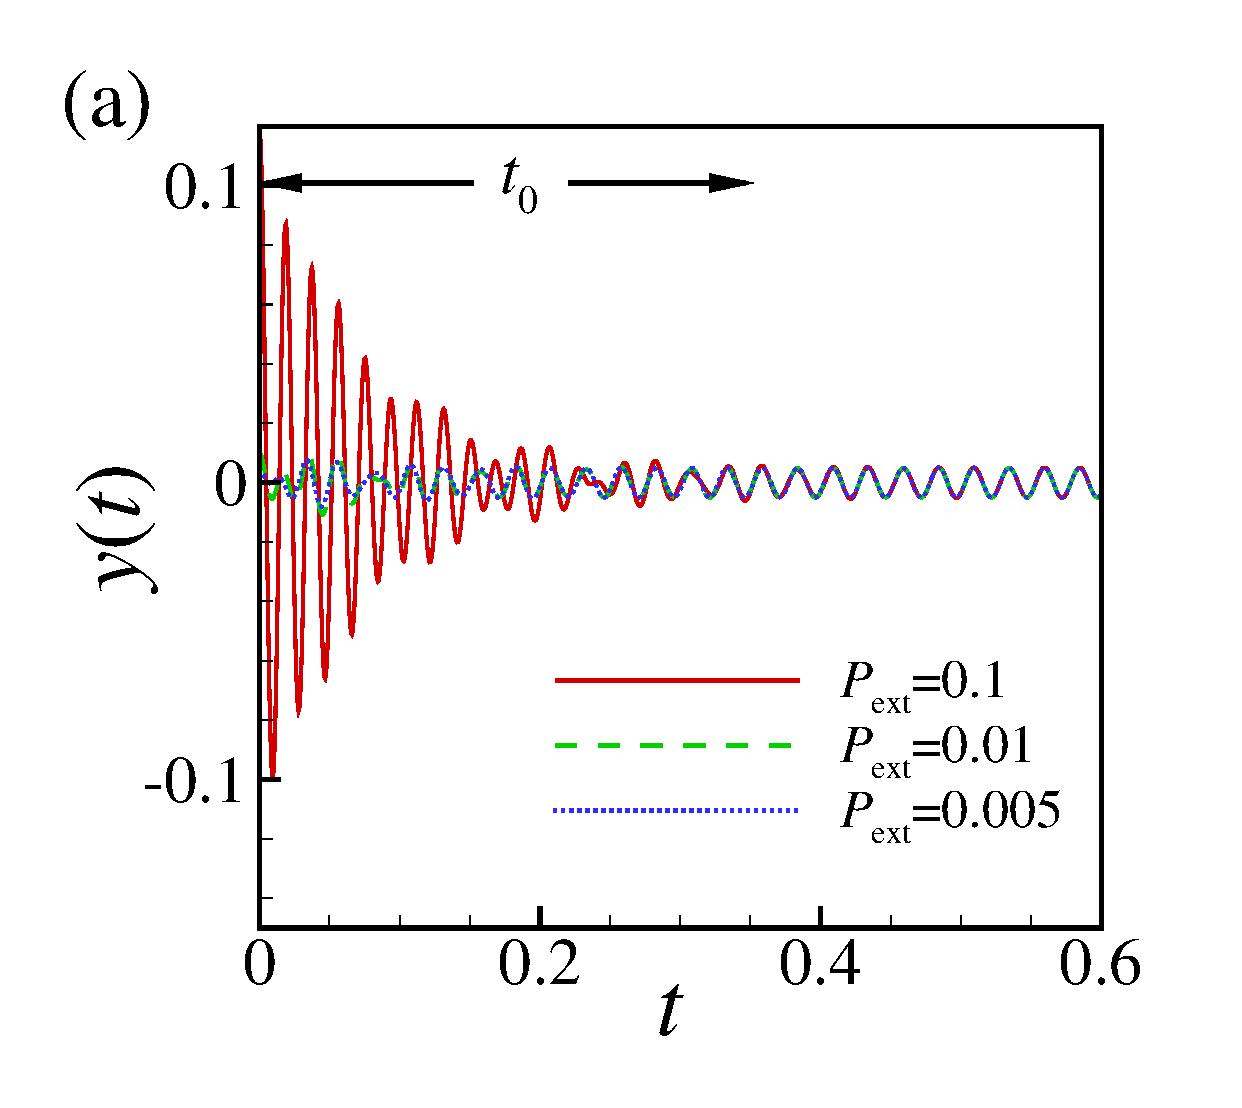
\includegraphics[width=0.49\linewidth, trim={0.5cm 0.5cm 1.5cm 0.5cm}, clip]{./epsFig/fig2a.eps}
\DIFdelbeginFL %DIFDELCMD < 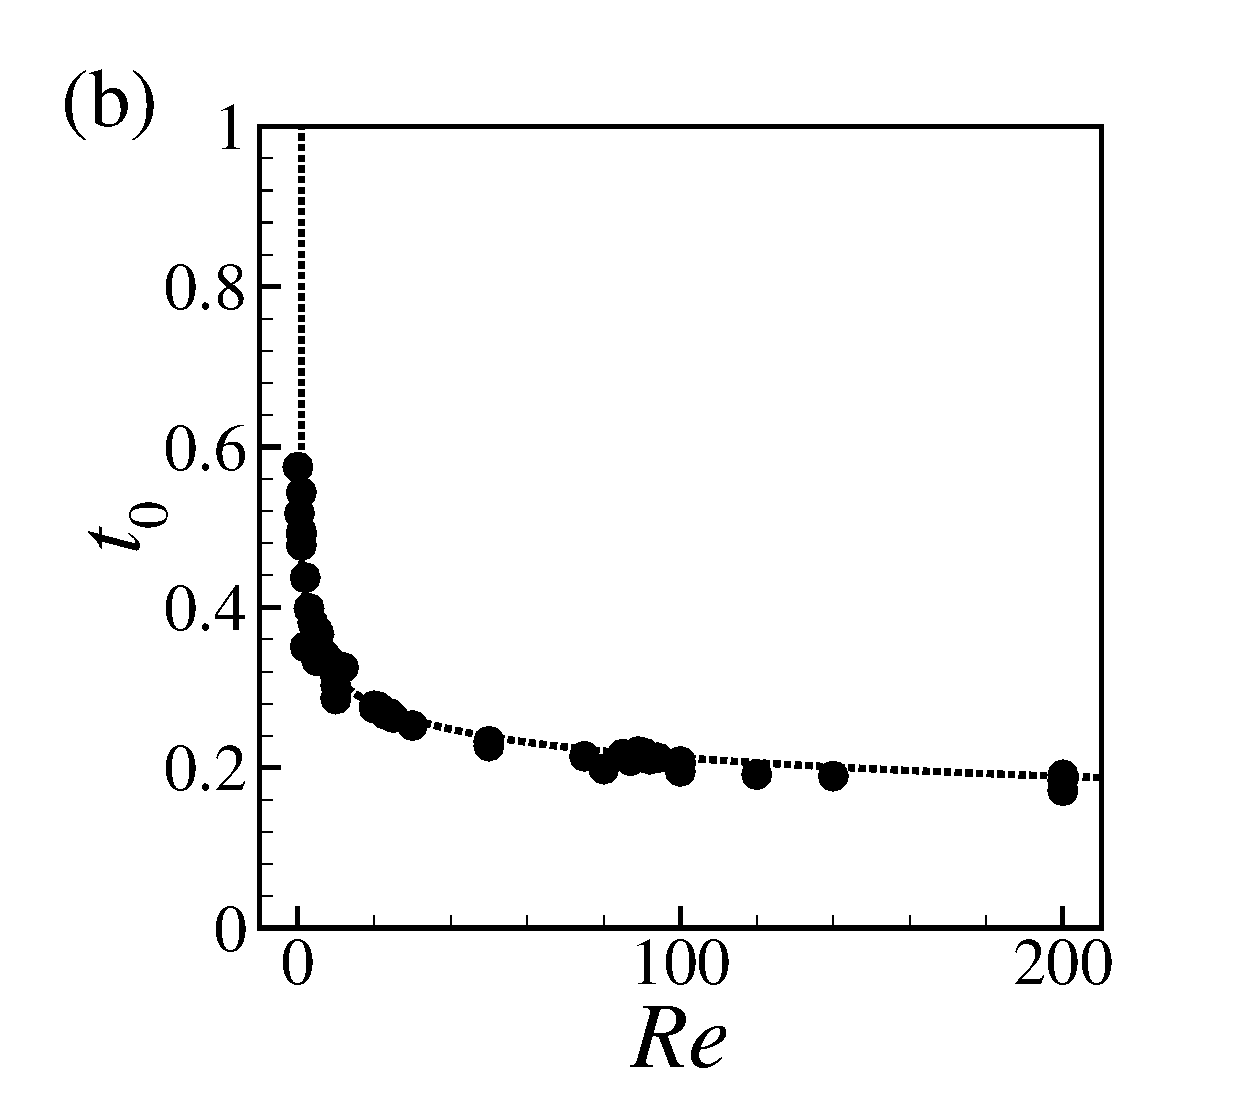
\includegraphics[width=0.49\linewidth, trim={0.5cm 0.5cm 1.5cm 0.5cm}, clip]{./epsFig/fig2b.eps}
%DIFDELCMD < %%%
\DIFdelendFL %DIF > 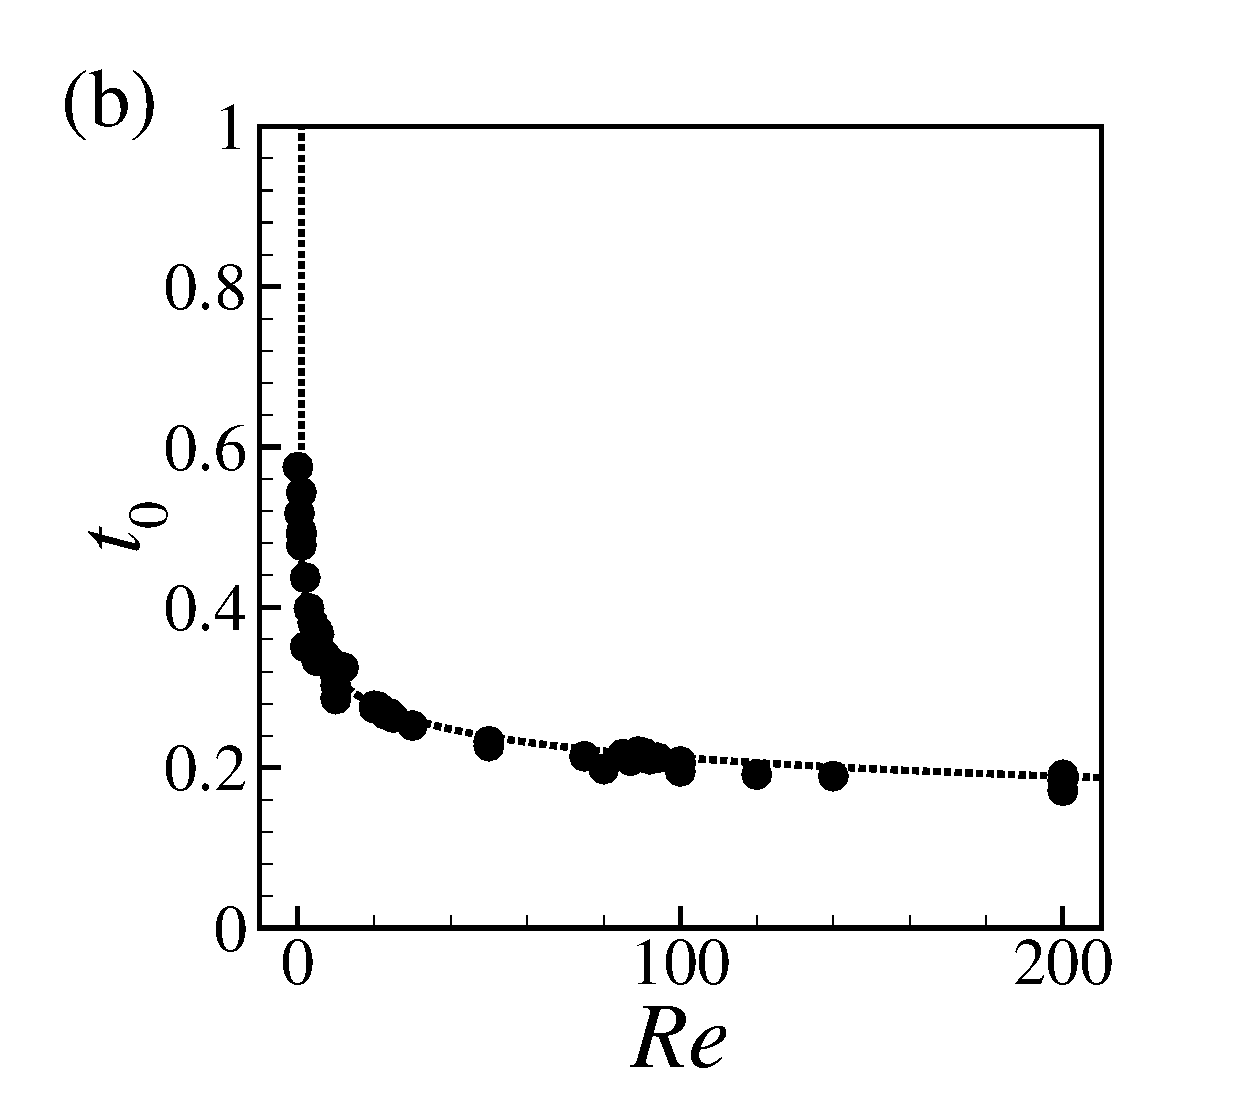
\includegraphics[width=0.49\linewidth, trim={0.5cm 0.5cm 1.5cm 0.5cm}, clip]{./epsFig/fig2b.ep}
  %DIF > 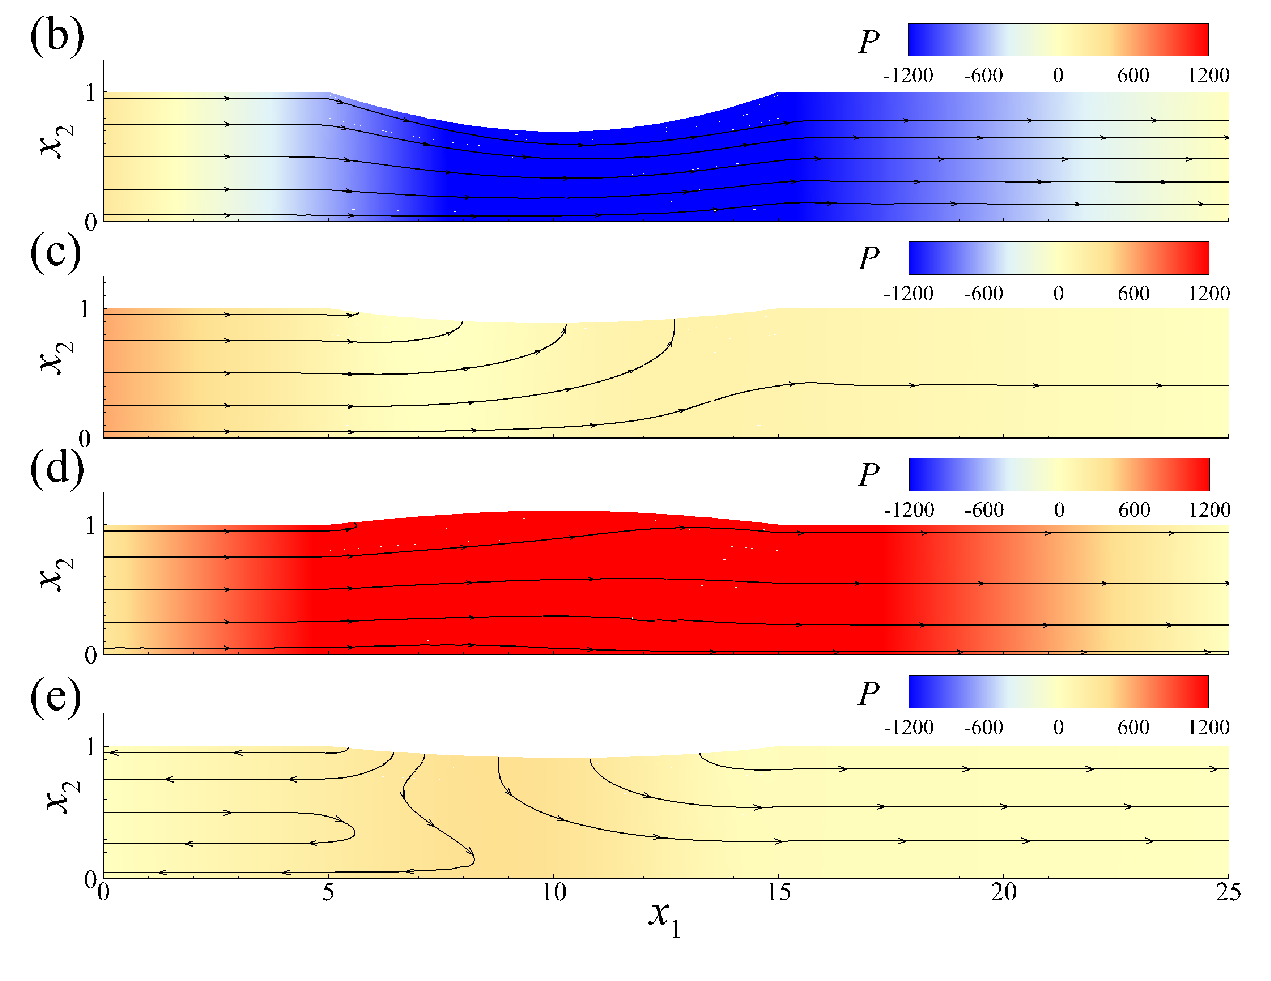
\includegraphics[width=1\linewidth, trim={0.2cm 0cm 0cm 0cm},
  %DIF > clip]{./epsFig/fig1b.eps}
  \DIFaddbeginFL 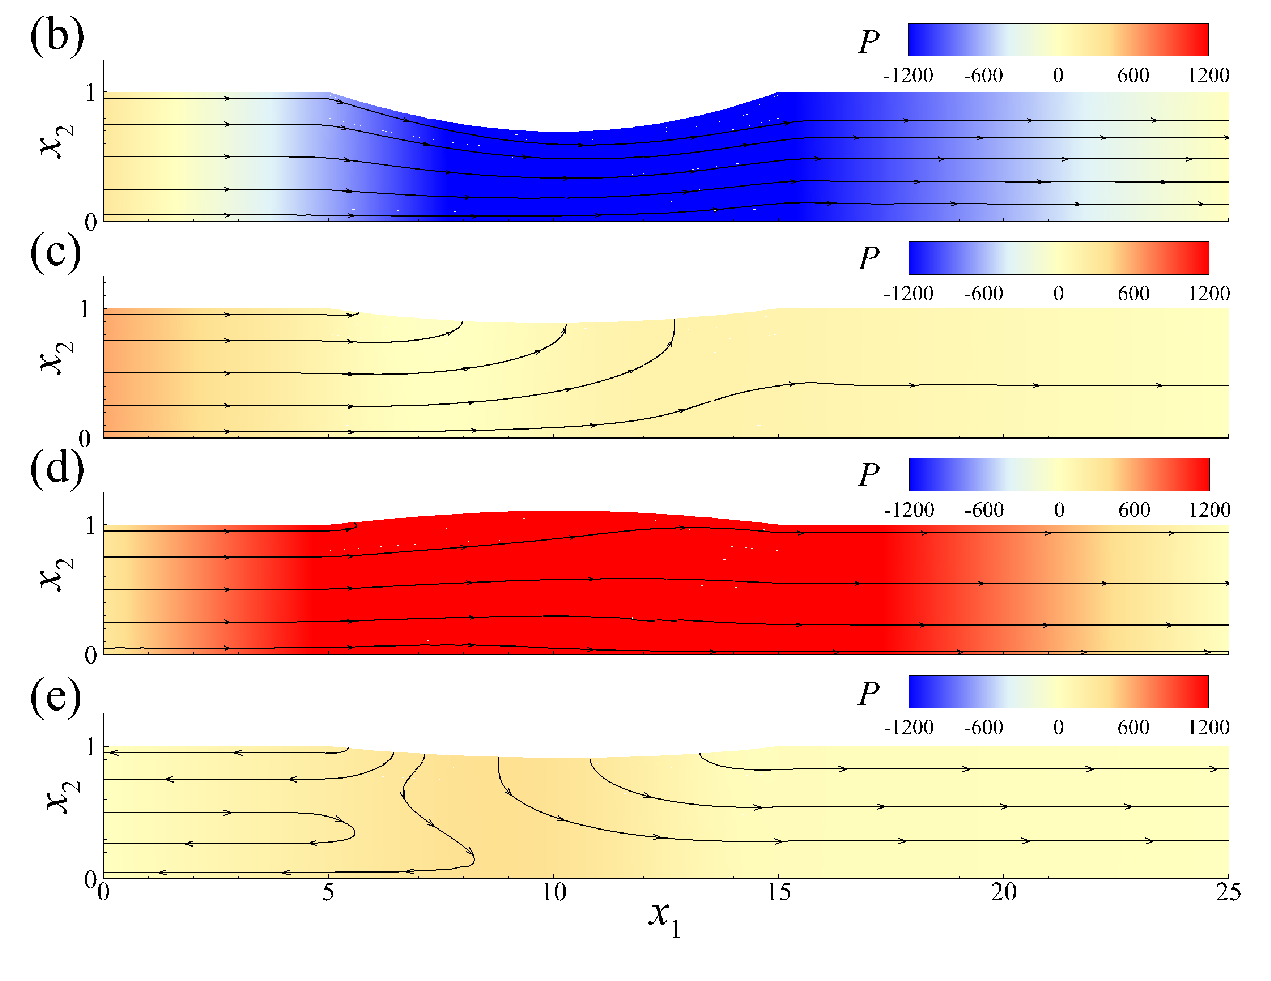
\includegraphics[width=1\linewidth]{./epsFig/fig1b.eps}
\DIFaddendFL \caption{\label{fig:extpressure}(Color online)  (a) Time \DIFdelbeginFL \DIFdelFL{series }\DIFdelendFL \DIFaddbeginFL \DIFaddFL{trace }\DIFaddendFL of \DIFaddbeginFL \DIFaddFL{the }\DIFaddendFL vertical
  displacement of the membrane \DIFdelbeginFL \DIFdelFL{at }\DIFdelendFL \DIFaddbeginFL \DIFaddFL{mid-point, $y(t)$, for }\DIFaddendFL $\Rey=50$, \DIFaddbeginFL \DIFaddFL{$\omega=***$,
  }{\bf \DIFaddFL{*** was }\DIFaddendFL $\Wo=15.81$, \DIFaddbeginFL \DIFaddFL{***}}
  \DIFaddendFL $Q=10^{-5}$,
  and \DIFaddbeginFL \DIFaddFL{for }\DIFaddendFL three different external pressures ($P_\text{ext}=0.1$, $0.01$
  and $0.005$)\DIFdelbeginFL \DIFdelFL{as a function of time}\DIFdelendFL . \DIFaddbeginFL \DIFaddFL{(b) }\DIFaddendFL The \DIFaddbeginFL \DIFaddFL{same data after subtracting the
  }\DIFaddendFL time-averaged displacements \DIFdelbeginFL \DIFdelFL{after }\DIFdelendFL \DIFaddbeginFL \DIFaddFL{$\overline{y}$ following the decay of the
  initial }\DIFaddendFL transients (\DIFdelbeginFL \DIFdelFL{$0.877$, $0.990$ }\DIFdelendFL \DIFaddbeginFL \DIFaddFL{$\overline{y} = 0.877, 0.990$ }\DIFaddendFL and $0.996$\DIFaddbeginFL \DIFaddFL{,
  respectively}\DIFaddendFL )\DIFdelbeginFL \DIFdelFL{are subtracted}\DIFdelendFL . \DIFaddbeginFL {\bf \DIFaddFL{*** Change y-axis labels accordingly ***}}
  \DIFaddendFL (\DIFdelbeginFL \DIFdelFL{b}\DIFdelendFL \DIFaddbeginFL \DIFaddFL{c-f}\DIFaddendFL ) \DIFdelbeginFL \DIFdelFL{Decay time }\DIFdelendFL \DIFaddbeginFL \DIFaddFL{Contour }\DIFaddendFL of \DIFdelbeginFL \DIFdelFL{initial transients $t_0$ at $P_\text{ext}=0.1$ }\DIFdelendFL \DIFaddbeginFL \DIFaddFL{pressure
  }\DIFaddendFL and \DIFdelbeginFL \DIFdelFL{$Q= 10^{-5}$ as function }\DIFdelendFL \DIFaddbeginFL \DIFaddFL{streamlines at four equally-spaced
  instants throughout the period }\DIFaddendFL of \DIFdelbeginFL \DIFdelFL{Reynolds number }\DIFdelendFL \DIFaddbeginFL \DIFaddFL{the time-periodic oscillation
  following the decay of the initial transients }\DIFaddendFL for \DIFdelbeginFL \DIFdelFL{$\Wo\in[0.32, 63.25]$}\DIFdelendFL \DIFaddbeginFL \DIFaddFL{$P_\text{ext}=0.1$}\DIFaddendFL .
  \DIFdelbeginFL \DIFdelFL{The dashed line shows }\DIFdelendFL \DIFaddbeginFL {\bf \DIFaddFL{*** where are }\DIFaddendFL the \DIFdelbeginFL \DIFdelFL{curve $0.423\,Re^{-1/6}$.}\DIFdelendFL \DIFaddbeginFL \DIFaddFL{additional
    plots? *** }}\DIFaddendFL }
  %DIF > (b) Decay time of initial transients $t_0$ at $P_\text{ext}=0.1$ and
  %DIF > $Q= 10^{-5}$ as function of Reynolds number for $\Wo\in[0.32,
  %DIF >   63.25]$. The dashed line shows the curve $0.423\,Re^{-1/6}$.}
\end{figure}
% Duo: Font size of the figures will be adjusted after we decide the position of the two panels to be left-right or top-bottom.
% Marc:
% Delete the inset in panel a
% Use left-right arrengement
% Use the same symbol for all data points in (b); ideally we would have simulations for a few selected Wo and show the symbols, but if we introduce St it becomes more confusing than it helps.
% Duo: done.

We \DIFdelbegin \DIFdel{investigated }\DIFdelend \DIFaddbegin \DIFadd{investigate }\DIFaddend the dynamics of the system by monitoring the vertical
displacement of the membrane at its midpoint\DIFaddbegin \DIFadd{, $y(t)$, }\DIFaddend as a proxy \DIFdelbegin \DIFdel{of }\DIFdelend \DIFaddbegin \DIFadd{for }\DIFaddend the
deformation. \DIFdelbegin \DIFdel{Initially, }\DIFdelend \DIFaddbegin \DIFadd{We start the simulations from an initial condition in
which }\DIFaddend the membrane is undeformed and the velocity
field is \DIFdelbegin \DIFdel{parabolic laminar }\DIFdelend \DIFaddbegin \DIFadd{steady }\DIFaddend Poiseuille flow. \DIFdelbegin \DIFdel{Subsequently, the external
pressure pushes the membrane inward andthis undergoes damped oscillations before settling }\DIFdelend \DIFaddbegin \DIFadd{For a sufficiently large external
pressure the membrane is pushed inwards and, following 
the decay of initial transients the system ultimately settles }\DIFaddend into a
time-periodic (\DIFaddbegin \DIFadd{approximately }\DIFaddend harmonic) motion \DIFdelbegin \DIFdel{. }\DIFdelend \DIFaddbegin \DIFadd{with the period of the
forcing, $2\pi/\omega$, about a mean value $\overline{y}$. This is
illustrated in }\DIFaddend Fig.~\ref{fig:extpressure}(a) \DIFaddbegin \DIFadd{which shows time traces of $y(t)$
for a range of external pressures. In Fig.~\ref{fig:extpressure}(b) we plot
the same data but subtract the time-average displacement
$\overline{y}$ following the decay of the initial transients. This }\DIFaddend shows
that the \DIFdelbegin \DIFdel{final }\DIFdelend amplitude of the \DIFdelbegin \DIFdel{membrane oscillations $y(t)$ }\DIFdelend \DIFaddbegin \DIFadd{time-periodic oscillation, $\widehat{y}$, }\DIFaddend is
independent of the external pressure \DIFdelbegin \DIFdel{, so from now }\DIFdelend \DIFaddbegin \DIFadd{(and from now on }\DIFaddend we set $P_\text{ext}=0.1$\DIFdelbegin \DIFdel{. }\DIFdelend \DIFaddbegin \DIFadd{).
}{\bf \DIFadd{*** DON'T UNDERSTAND THE FOLLOWING SENTENCE ``}\DIFaddend Note that this
behavior is in contrast to self-excited oscillations generated by a
constant pressure gradient \cite{Tang15}.\DIFaddbegin \DIFadd{'' HOW CAN A CONSTANT
PRESSURE
GRADIENT GENERATED OSCILLATIONS; IF THEY'RE SELF-EXCITED THEN IT'S
A TOTALLY DIFFERENT PROBLEM! KILL?***}}
\DIFaddend The duration of the initial transients \DIFdelbegin \DIFdel{$t_0$ }\DIFdelend is on the order of \DIFdelbegin \DIFdel{a }\DIFdelend \DIFaddbegin \DIFadd{the
}\DIFaddend viscous time unit, \DIFdelbegin \DIFdel{suggesting }\DIFdelend \DIFaddbegin \DIFadd{$\nu/a^2$, which, in our non-dimensionalisation
is equal to the Reynolds number, ${\cal T}_{\rm visc} = Re$. This suggests
}\DIFaddend that the adjustment toward a \DIFdelbegin \DIFdel{harmonic oscillation is 
predominantly }\DIFdelend \DIFaddbegin \DIFadd{time-periodic oscillation is 
}\DIFaddend controlled by the viscosity of \DIFdelbegin \DIFdel{fluid. Overall, $t_0$ is largely unaffected by the pulsation frequency and diminishes slowly as $\Rey$ increases (see Fig. ~\ref{fig:extpressure}b) . 
}\DIFdelend \DIFaddbegin \DIFadd{the fluid.
}

\DIFadd{Figs. \ref{fig:extpressure}(c-f) illustrate... }{\bf \DIFadd{*** Note: these plots were
  never discussed in the original version of the manuscript. Important
  to stress that the system undergoes large deflections and that there's
  significant FSI -- the motion of the membrane induces large sloshing
flows, etc. However, are these plots the right ones to show here? The amplitude
seems larger than that displayed in the time trace. Can we use some
that match the time traces?}}
\DIFaddend 

\begin{figure}
\centering
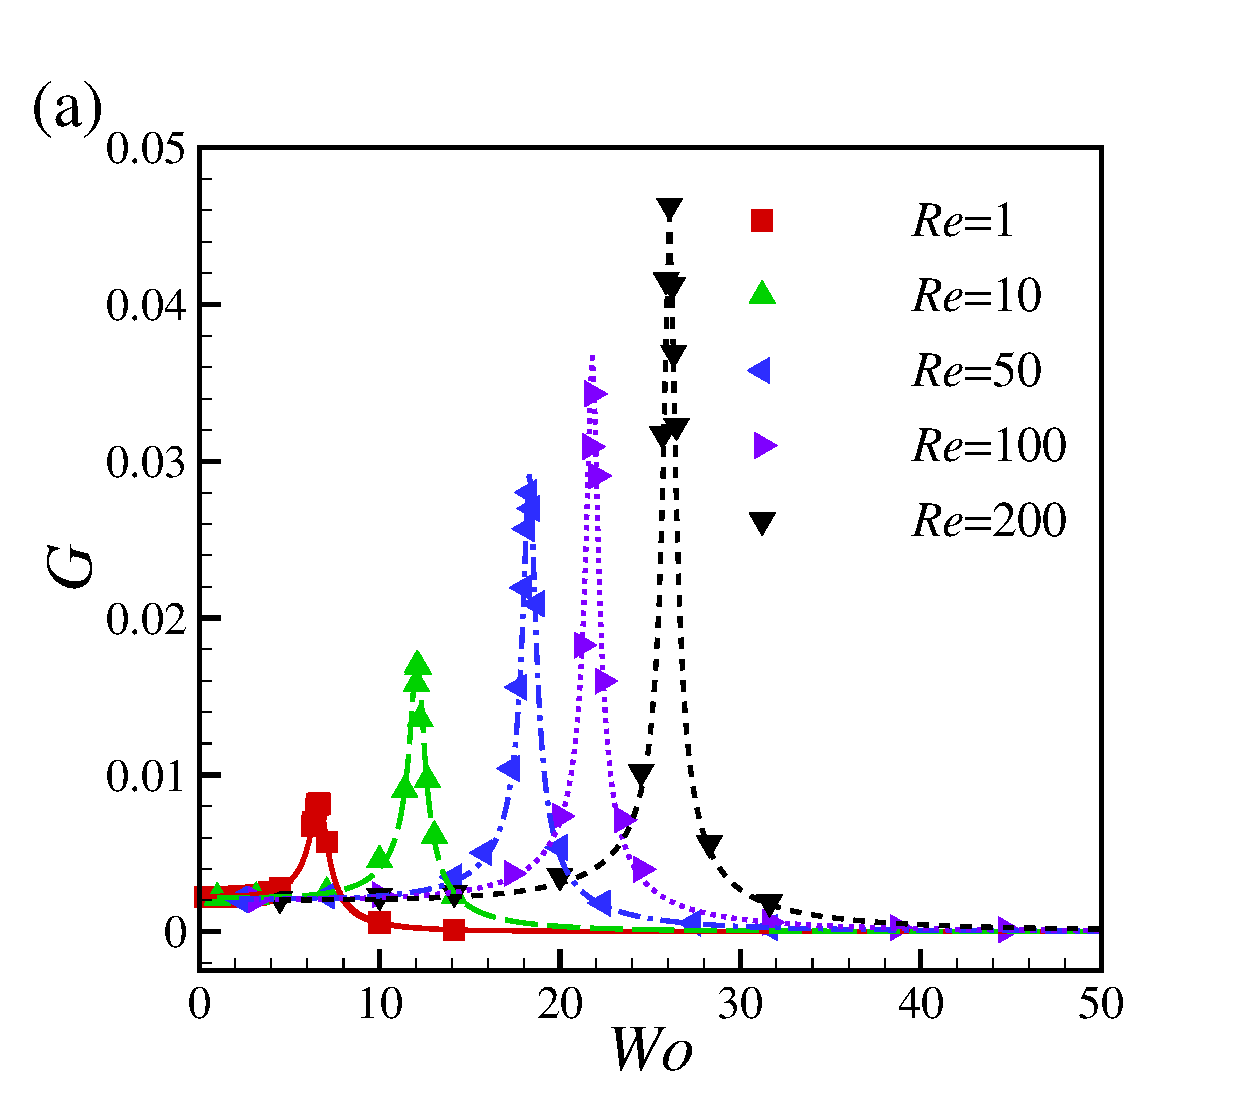
\includegraphics[width=0.49\linewidth, trim={0.3cm 0cm 1.75cm 1cm}, clip]{./epsFig/fig3a.eps}	
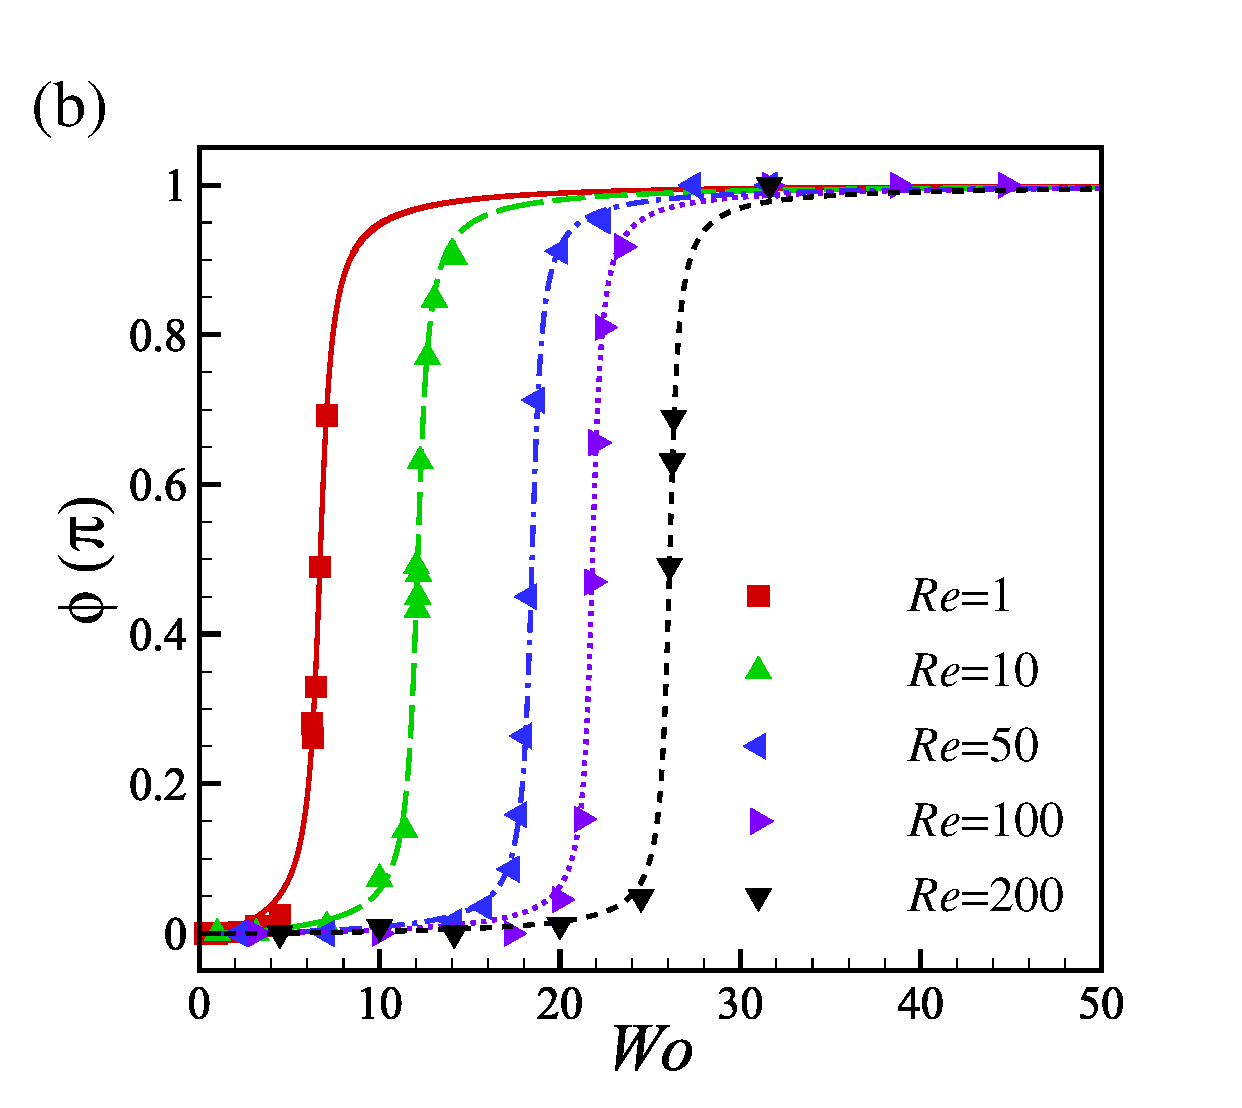
\includegraphics[width=0.49\linewidth, trim={0.3cm 0cm 1.75cm 1cm}, clip]{./epsFig/fig3b.eps}
\caption{\label{fig:amplitude_phase}(Color online) (a) Amplitude of
  the steady-state oscillations\DIFaddbeginFL \DIFaddFL{, $\widehat{y}$, }\DIFaddendFL as a function of
  \DIFdelbeginFL \DIFdelFL{$Wo$ }\DIFdelendFL \DIFaddbeginFL \DIFaddFL{$\omega$ }\DIFaddendFL for several $Re$ as indicated in the legend.
  Here $P_\text{ext}=0.1$ and \DIFdelbeginFL \DIFdelFL{$Q=10^{-5}$}\DIFdelendFL \DIFaddbeginFL \DIFaddFL{$H=***$}\DIFaddendFL . (b) Phase shift $\phi$ as a
  function \DIFdelbeginFL \DIFdelFL{$\Wo$}\DIFdelendFL \DIFaddbeginFL \DIFaddFL{$\omega$}\DIFaddendFL . Symbols denote the simulation data and lines are
  from the harmonic oscillator model, with eq.~\eqref{eq:channel_gain}
  for \DIFdelbeginFL \DIFdelFL{$G$  }\DIFdelendFL \DIFaddbeginFL \DIFaddFL{$\widehat{y}$ }\DIFaddendFL and \eqref{eq:channel_phase} for $\phi$, respectively.}
\end{figure}

We now focus on the dynamics of the steady-state oscillations \DIFdelbegin \DIFdel{after transients. The symbols in }\DIFdelend \DIFaddbegin \DIFadd{following
the decay of the transients. }\DIFaddend Fig.~\ref{fig:amplitude_phase}(a) shows the
amplitude of the oscillations\DIFdelbegin \DIFdel{$G$ against $\Wo$ }\DIFdelend \DIFaddbegin \DIFadd{, $\widehat{y}$, against the
non-dimensonal forcing frequency $\omega$ }\DIFaddend for five different
Reynolds numbers \DIFdelbegin \DIFdel{and $Q=10^{-5}$.
As the driving frequency increases, the oscillation }\DIFdelend \DIFaddbegin \DIFadd{while keeping $H = Re/Q = ****$ constant.
The }\DIFaddend amplitude of the membrane \DIFdelbegin \DIFdel{first increases and then decreases. Note also that there is a phase shift }\DIFdelend \DIFaddbegin \DIFadd{oscillation has a sharp maximum at
$\omega_0 \approx ***$, irrespective of the Reynolds number. Furthermore,
the phase }\DIFaddend $\phi$ \DIFdelbegin \DIFdel{between $\Delta P(t)$ and }\DIFdelend \DIFaddbegin \DIFadd{between the forcing pressure, $P(t)$, and }\DIFaddend $y(t)$ \DIFdelbegin \DIFdel{, which depends on $\Wo$. In all cases, when the amplitude of the response features a sharp peak,
the pressure difference and membrane displacement are exactly out of phase ($\phi=\pi/2$).  
}\DIFdelend \DIFaddbegin \DIFadd{varies
with $\omega$ and displays a $180^{o}$ phase shift when $\omega$
passes through $\omega_0.$ }{\bf \DIFadd{*** please do these computations and
  update figures ***}}
\DIFaddend 

\DIFdelbegin \DIFdel{The response of the membrane deformation }\DIFdelend \DIFaddbegin \DIFadd{This behaviour }\DIFaddend is reminiscent of the response of the forced damped
harmonic oscillator\DIFaddbegin \DIFadd{...
}



\hrule
\newpage



\DIFaddend in classical mechanics \cite{Shabana91}, which consists of a mass $\widetilde{m}$ attached to a spring with stiffness coefficient $\widetilde{k}$ subject to an external harmonic force of amplitude $\widetilde f$ and frequency $\omega$. In addition, the motion of the mass is damped by viscous force with damping coefficient $c$. The governing equation of the harmonic oscillator is
\begin{equation}
\widetilde m\frac{\partial^2 \widetilde y}{\partial {\widetilde t}^2}=-c\frac{\partial \widetilde y}{\partial \widetilde t}-\widetilde k\,\widetilde y+\widetilde f\sin  \omega \widetilde t,
\label{eq:oscillator_eqn}
\end{equation}	
where $\widetilde y$ is the instantaneous displacement of the mass with respect to the equilibrium position. In what follows, we explore an analogy between the collapsible channel driven by a pulsatile pressure difference and the driven harmonic oscillator. In this analogy, the displacement of the membrane's midpoint $y(t)$ is assumed to exhibit dynamics similar to the spring displacement $\widetilde y(t)$ in the harmonic oscillator. 

In our model, the spring constant $k$ is assumed proportional to the effective Young modulus of the membrane and to its length, i.e.~$\tilde k=A_\text{k}\, E_\text{eff}\,l_\text{m}$, whereas the mass is assumed proportional to the mass of fluid beneath the membrane $\tilde m=A_\text{m}\, \rho\, l_\text{m}\, h^2$. The main driving force is expected to be proportional to the pressure force acting on the membrane $\tilde f=A_\text{f}\,\rho\nu\, \bar{u}\, l_\text{m}$. Note that because the flow is laminar, we choose the viscous scale $\rho\nu\, \bar{u}/h$ for the pressure. The scaling of the viscous damping coefficient $c$ is unclear a priori, so this is left as unknown for the time being. 

Plugging in the expressions for $\tilde m$,  $\tilde f$ and $\tilde k$ above into \eqref{eq:oscillator_eqn} and rendering the equation dimensionless by rescaling lengths with $h$, velocities with $\bar{u}$ and time with $h^2/\nu$, we obtain the following model 
\begin{equation}
\frac{\partial^2 y}{\partial t^2}+C_\text{d}\frac{\partial y}{\partial t}+\left(\Wo^4_0\right)y={\alpha_f}{\Rey}\;\sin\left(\Wo^2 \, t\right),
\label{eq:channel_eqn}
\end{equation}
with $\alpha_f=A_\text{f}/A_\text{m}$ and the drag coefficient $C_\text{d}=c/(A_\text{m}\,\rho\nu\,l_\text{m})$. The model predicts that the eigenfrequency $\Wo_0$ of the collapsible channel depends on the material properties of the fluid-structure interaction as
\begin{equation}\label{eq:model_St0}
\Wo_0=({\alpha_k}H)^{1/4},
\end{equation}
with the constant $\alpha_k=A_\text{k}/A_\text{m}$. The accuracy of the assumptions in our model can be assessed by fitting the simulation data with the well-known analytic steady-state solution of \eqref{eq:channel_eqn} 
\begin{equation}
y(t)=G \DIFdelbegin \DIFdel{\cdot}\DIFdelend \text{sin}\left(\Wo^2  \DIFdelbegin \DIFdel{\cdot }\DIFdelend t-\phi\right),
\label{eq:channel_solution}
\end{equation}
where 
\begin{equation}
G = \dfrac{{\alpha_f}{\Rey}}{\sqrt{\left(\Wo^4_0-\Wo^4\right)^2+C_\text{d}^2\,\Wo^4}},
\label{eq:channel_gain}
\end{equation}
is the amplitude of the oscillations (typically referred to as gain) and 
\begin{equation}
\phi=\tan^{-1}\left[\dfrac{C_\text{d}\, \Wo^2}{\Wo_0^4-\Wo^4}\right]
\label{eq:channel_phase}
\end{equation}
is the phase delay between driving force and response. In summary, there are three fit parameters, of which two ($\alpha_k$ and $\alpha_f$) should be constant according to the model, whereas the drag coefficient $C_\text{d}$ is expected to depend on the flow parameters and particularly on the Reynolds number. 

\begin{figure}
	\centering
	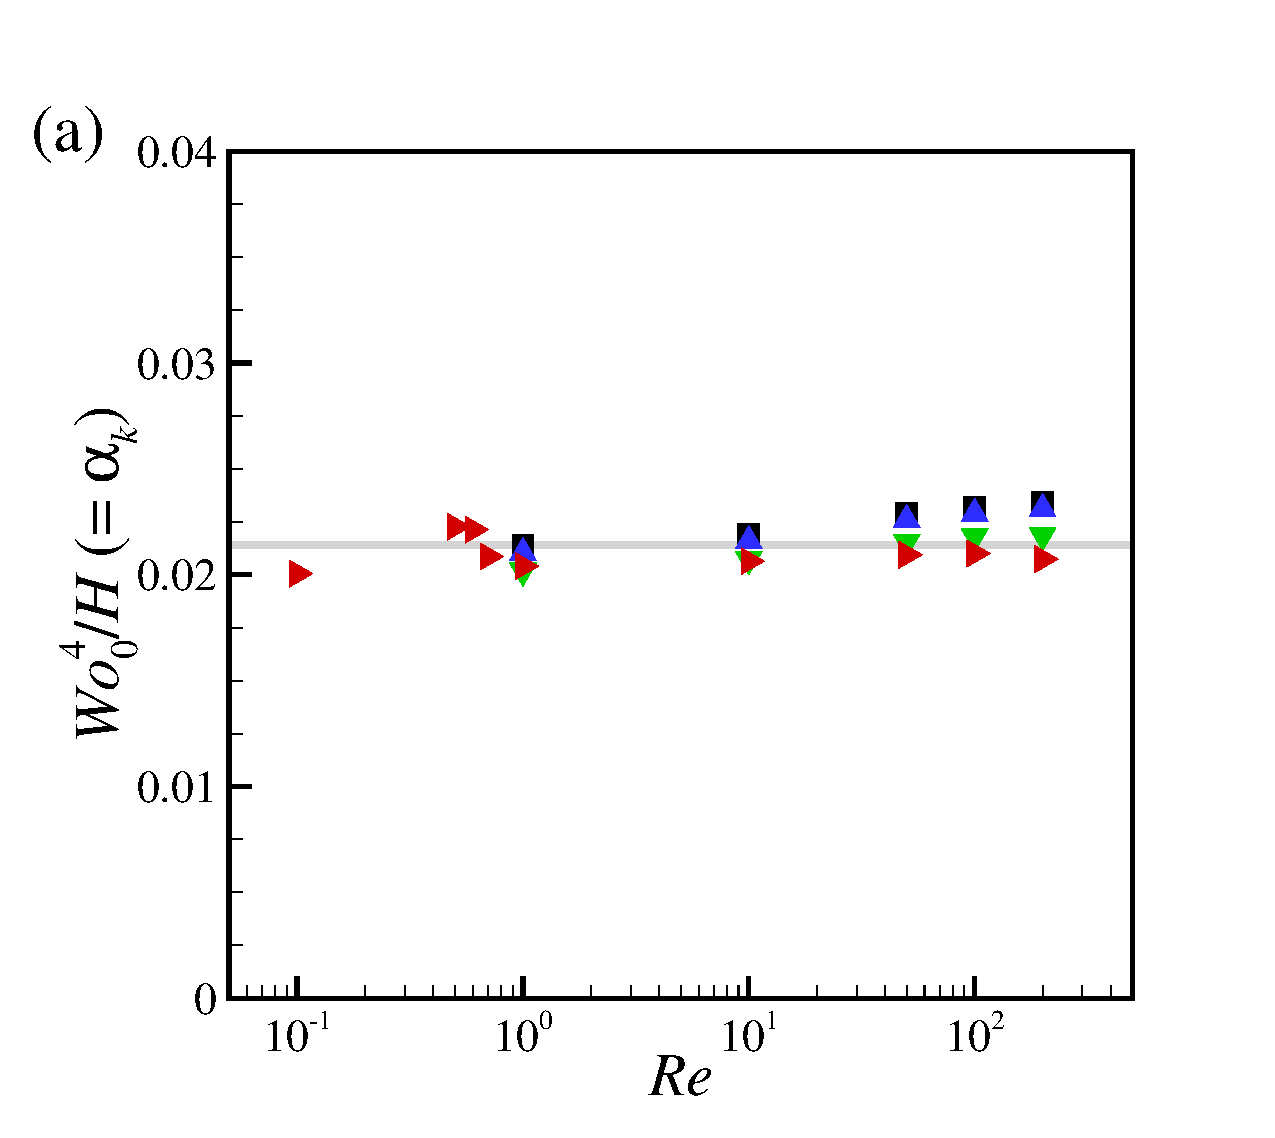
\includegraphics[width=0.49\linewidth, trim={0.25cm 0cm 1.5cm 1.5cm}, clip]{./epsFig/fig4a.eps}
	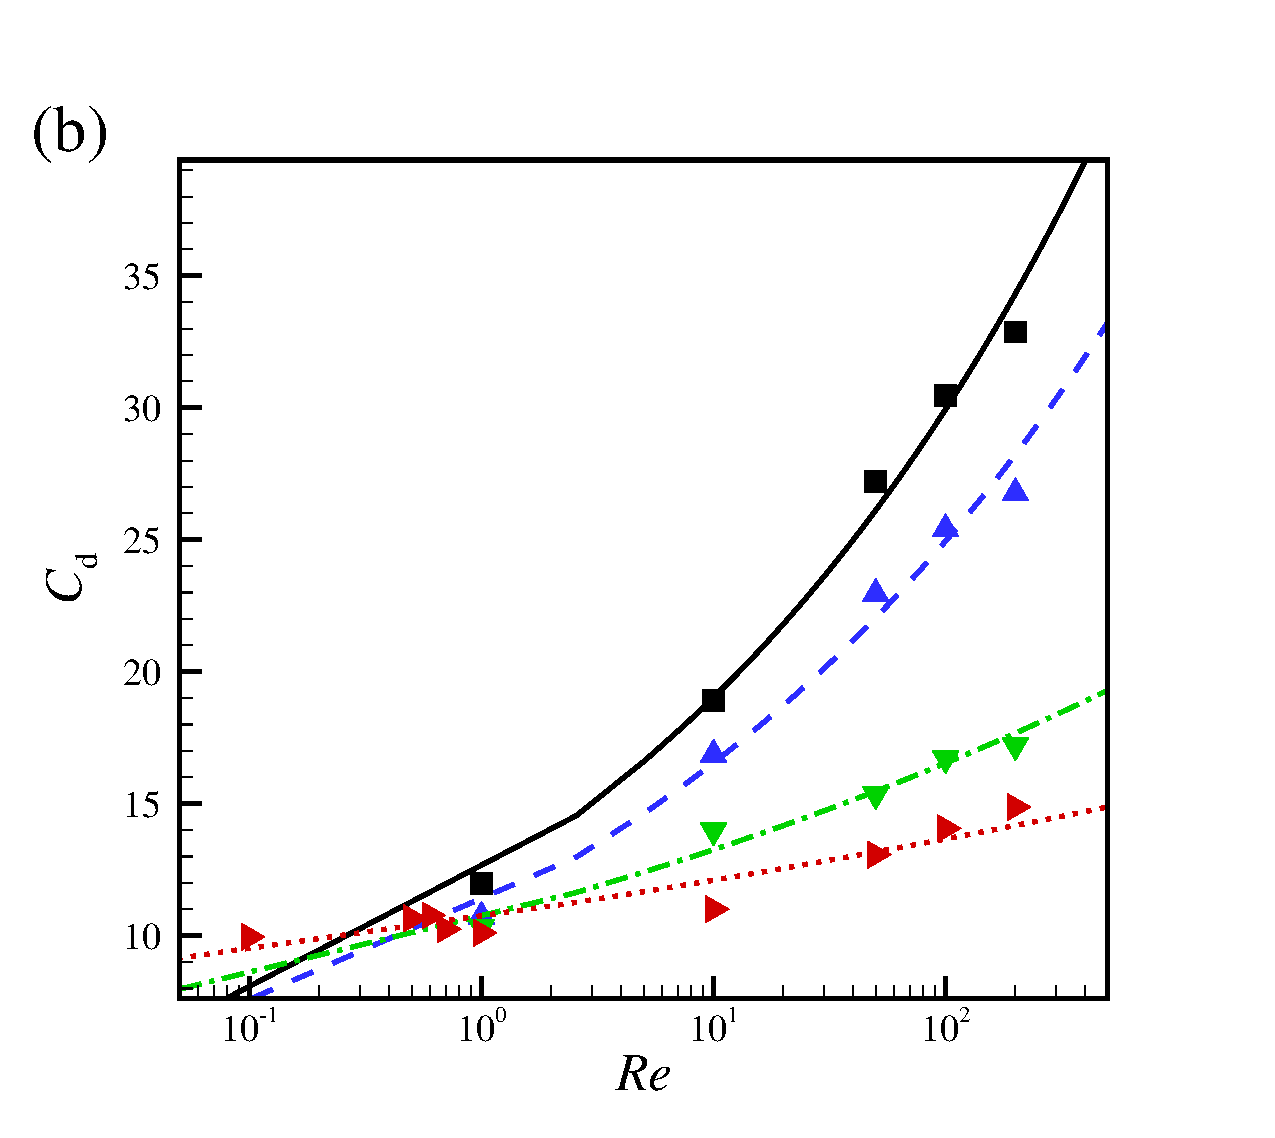
\includegraphics[width=0.49\linewidth, trim={0.25cm 0cm 1.5cm 1.5cm}, clip]{./epsFig/fig4b.eps}
	\caption{\label{fig:Wo0}(Color online) (a) Dimensionless eigenfrequency $\Wo_0$ of the collapsible channel against $\Rey$ for $Q=10^{-5}$ (black squares and black circles), $Q=2 \times 10^{-5}$ (blue up-triangles), $Q=10^{-4}$ (green down-triangles) and $Q=2\times10^{-4}$ (red right-triangles). The gray solid-line shows $\alpha_k=0.02$.	 
	% When I look at the figure is seems to me like the value of \alpha_k should be more like 0.025. How as this obtained?	
	(b) The drag coefficients $C_\text{d}$ varying with $Re$ where the symbols, the same as Fig.~\ref{fig:Str_Rer_Q}, lines are from power law fitting.
	%denote simulation results and the lines are $C_\text{d}=48\Rey(5\Rey)^{g(Q)}$, with $g(Q)=-1.475Q^{0.0495}$ (see Fig X in the supplementary materials). 
	% This figure needs to be redone with a more reasonable y axis. 
	}
\end{figure}


The lines in Fig.~\ref{fig:amplitude_phase}a show the best fits of the gain \eqref{eq:channel_gain} to the oscillation amplitude obtained from the numerical simulations. Indeed, we find that $\alpha_f\approx4.2$ and $\alpha_k\approx0.02$ % Are you sure that you are using this value? When I look into figure 4a, to me it seems more that the value should be 0.025 (it should agree well with the black data points). % Duo: the mean of alpha_k over four sets is 0.0215.
are constants adjusting all data sets, whereas $C_\text{d}$ depends on $\Rey$. The fitted values of $\alpha_f$, $\alpha_k$ and $C_\text{d}$ also render excellent approximations of the phase delay (see lines in Fig.~\ref{fig:amplitude_phase}b). Together these results suggest that the dynamics of the pulsatile collapsible channel can be accurately modeled with a harmonic oscillator. Despite the wide ranges of $\Wo$ and $\Rey$ covered in Fig.~\ref{fig:amplitude_phase}, all these simulations were obtained for $Q=10^{-5}$. This raises the question of whether the model captures the dependency on $Q$ as well, which was investigated here by performing additional sets of simulations for $Q=2\times 10^{-5}$, $10^{-4}$ and  $2\times 10^{-4}$.  Of particular interest is the eigenfrequency prediction (see \ref{eq:model_St0} and recall that $H=Re/Q$). Figure~{fig:Wo0}a confirms our prediction and shows that the eigenfrequency of the collapsible channel depends only on material parameters at low Reynolds numbers $\Rey\le 10$, whereas at higher $\Rey$ small but noticeable differences among the data sets for different $Q$ are observed. On the other hand, the data reveal a complex dependence of the friction coefficient on $\Rey$ and $Q$. In particular, $C_\text{d}$ follows a power-law of the Reynolds number, in which both pre-factor and exponent depend on $Q$ (see Fig.~\ref{fig:Wo0}b). 

\begin{figure}
	\centering	
	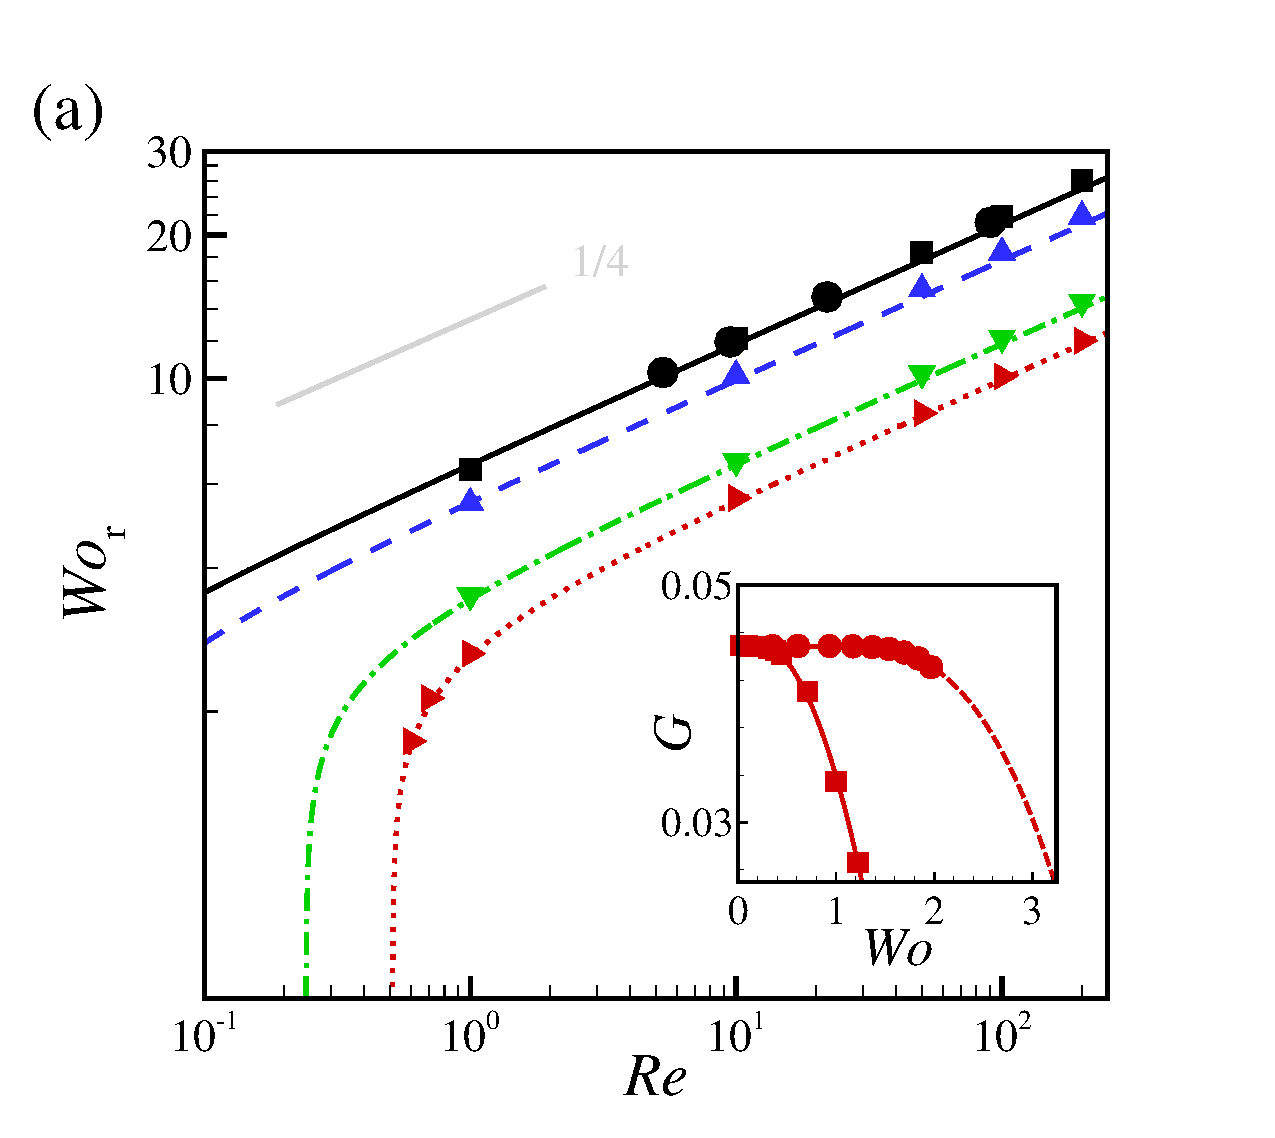
\includegraphics[width=0.49\linewidth, trim={0.25cm 0cm 1.5cm 1cm}, clip]{./epsFig/fig5_sub_a.eps}
	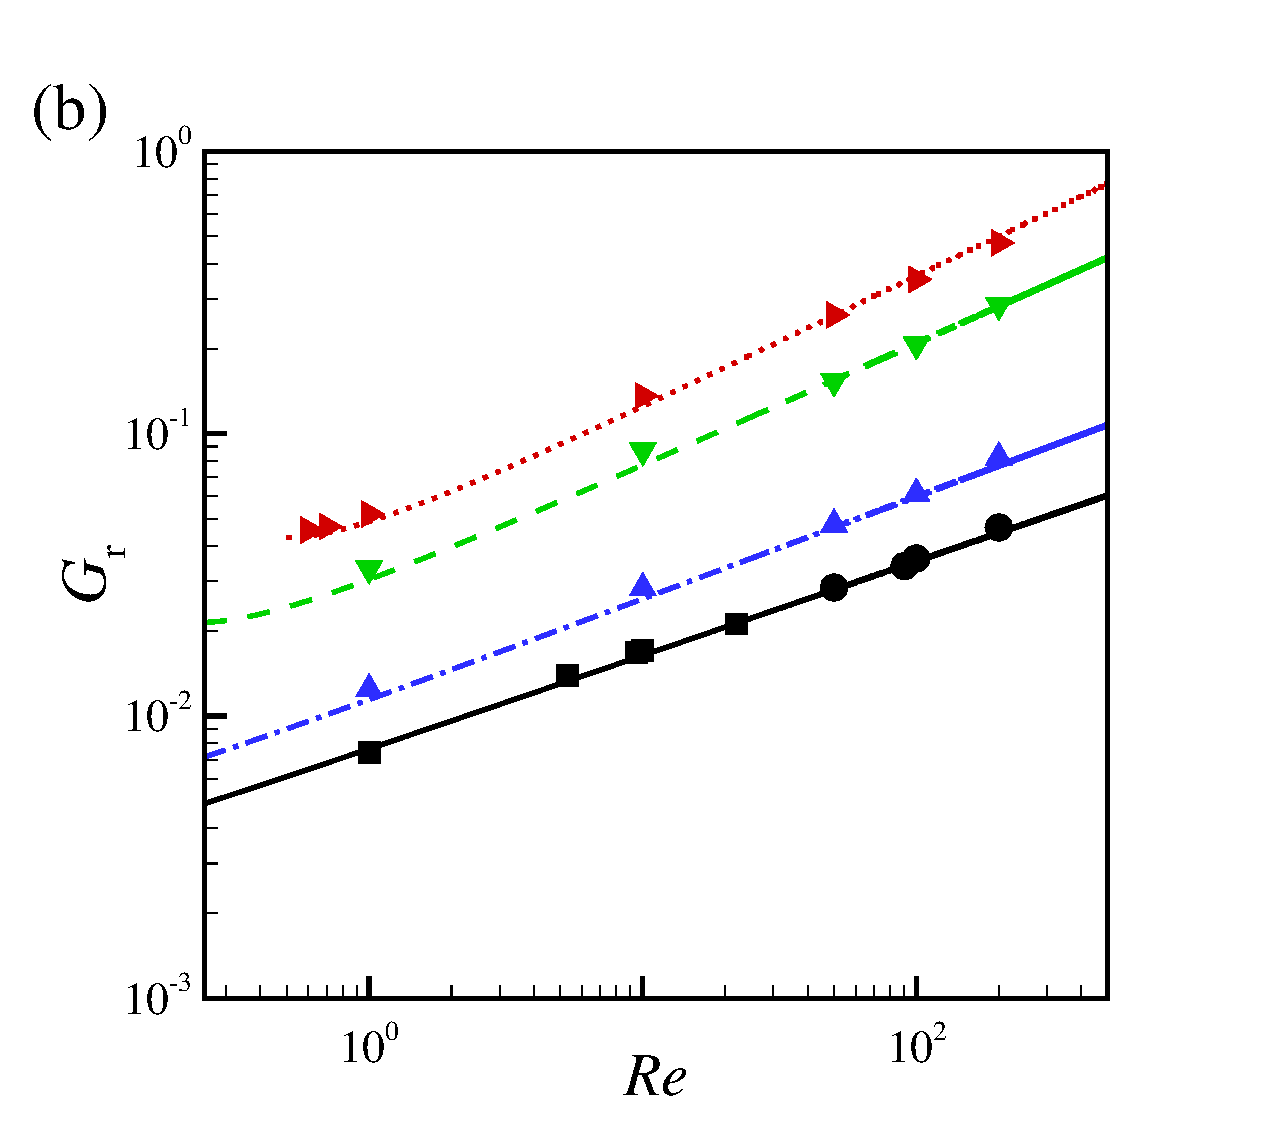
\includegraphics[width=0.49\linewidth, trim={0.25cm 0cm 1.5cm 1cm}, clip]{./epsFig/fig5b.eps}
	\caption{\label{fig:Str_Rer_Q} (Color online)  (a) Resonant points for $Q=10^{-5}$ (black squares and black circles), $Q=2 \times 10^{-5}$ (blue up-triangles), $Q=10^{-4}$ (green down-triangles) and $Q=2\times10^{-4}$ (red right-triangles). The lines correspond to Eq.~\ref{eq:channel_gain} and \ref{eq:St_resonance} with $\alpha_f=4.2$ and $\alpha_k=0.02$. (a) $(\Rey, \Wo_\text{r})$, where the inset shows that for $Q=2\times10^{-4}$ at $\Rey=0.1$ (squares) and $0.5$ (circles) $G$ increases and saturates at a constant as $\Wo$ decreases. (b) The oscillation amplitudes $G_\text{r}$ against the Reynolds number $\Rey$ at the resonance.}
\end{figure}

A well-known feature of the driven harmonic oscillator is that resonances disappear as the damping increases. More specifically, the resonant Womersley number
\begin{equation}
\Wo_\text{r}=(\Wo^4_0-C_\mathrm{d}^2/2)^{1/4},
\label{eq:St_resonance}
\end{equation}
maximizing the gain $G$ (in Eq.~\ref{eq:channel_gain}) disappears when $C_\text{d} \geqslant \sqrt{2}\Wo^2_0$. This process of extinction of resonances occurs also in the collapsible channel. Figure~\ref{fig:Str_Rer_Q}a shows that as $C_\text{d}$ increases, the resonance peak becomes wider until it disappears. When this happens the maximum gain is oobtained in the quasi-static limit $\Wo\rightarrow 0$ (see inset of Fig.~\ref{fig:Str_Rer_Q}a). When $C_\text{d} \ll \sqrt{2}\Wo^2_0$, the resonant frequency is close to the eigenfrequency ($\Wo_\text{r}\approx\Wo_0$), and in view of Eq.~\ref{eq:model_St0}, $\Wo_\text{r}\propto \Rey^{1/4}$, as exhibited by our data (see the gray line in Fig.~\ref{fig:Str_Rer_Q}a). In this scaling regime, the maximum (resonant) gain $G_r \propto C_\text{d}^{-2}$  becomes a $Q$-dependent power-law of the Reynolds number, with exponent $0.33$ to $0.42$ as $Q$ increases from $10^{-5}$ to $2\times10^{-4}$. 

\begin{figure}
\centering
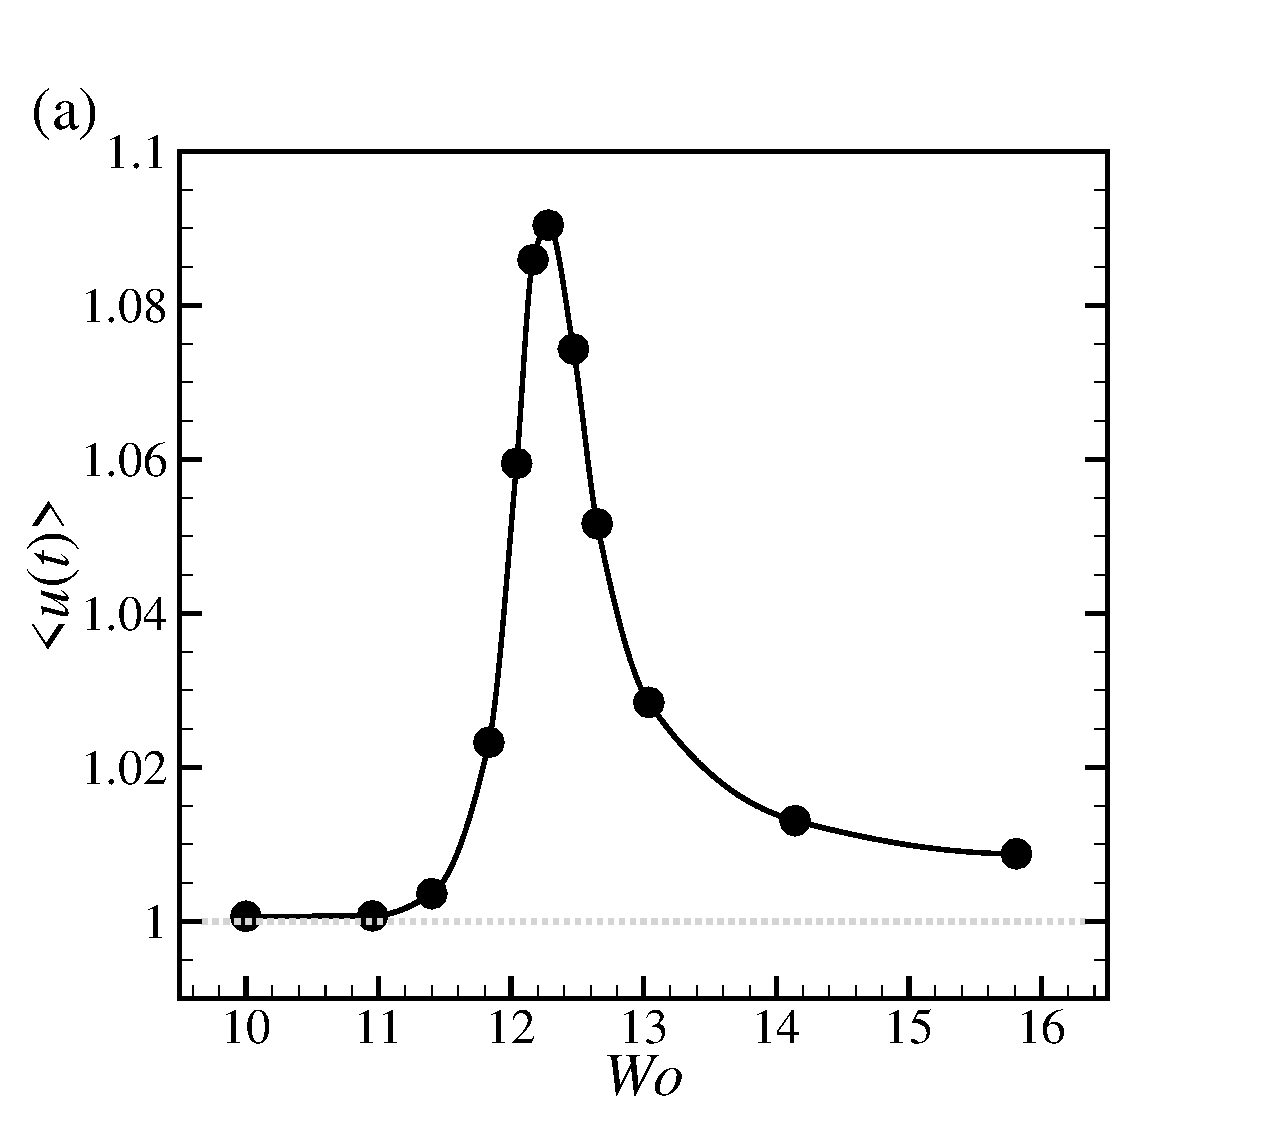
\includegraphics[width=0.49\linewidth, trim={0.2cm 0.4cm 0.4cm 0.5cm}, clip]{./epsFig/fig6a.eps}
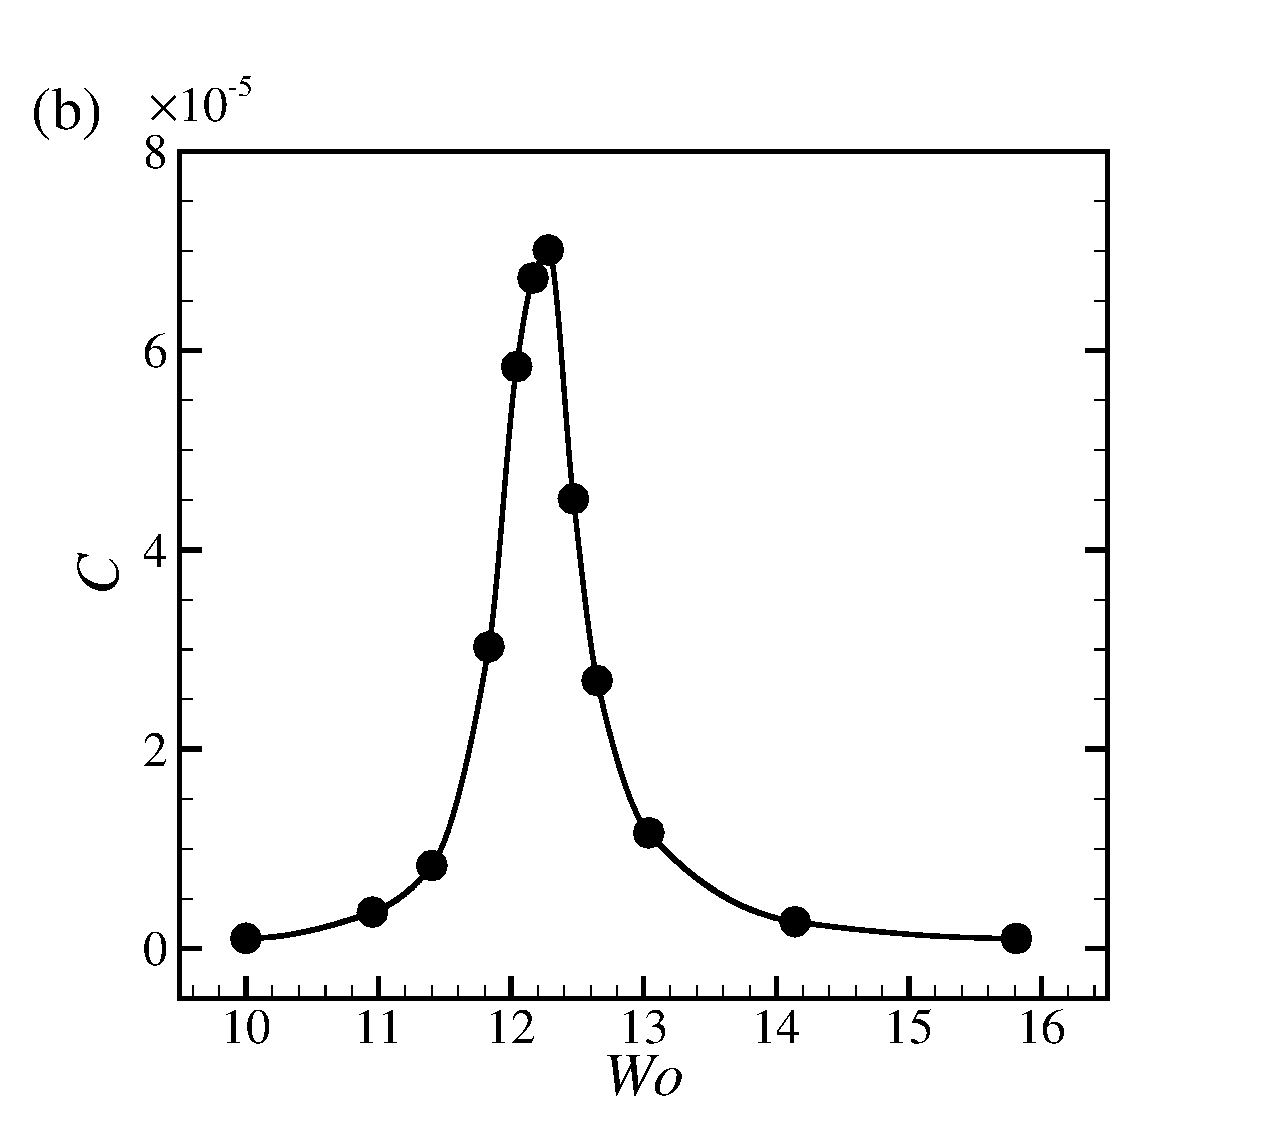
\includegraphics[width=0.49\linewidth, trim={0.2cm 0.4cm 0.4cm 0.5cm}, clip]{./epsFig/fig6b.eps}
\caption{(Color online) (a) Averaged streamwise fluid velocity $\langle u(t) \rangle$ against Womersley number $\Wo$ for $\Rey=100$, $Q=10^{-4}$ ($H=10^6$) and  $P_\mathrm{ext}=0.012$. (b) Flow compliance.}	\label{fig:flowrate_compliance}
\end{figure}
% Do not use Q for the flow rate (it may be confused with the other Q); actually this is the mean velocity
% Duo: changed.

The relationship between the driving pressure difference and the flow rate is important for fluid transport and has attracted much attention in studies of blood flows, where it is usually described with windkessel models \citep{Westerhof2009}.  %Citation is needed here % high citation paper
Figure~\ref{fig:flowrate_compliance}a shows the time-averaged streamwise velocity as a function of the Wommersly number. Here all other parameters were kept fixed, so that this figure illlustrates the effect of changing the pulsation frequency in a physical experiment. The external pressure was chosen such that the membrane oscillated with zero average deformation (i.e.\ about the height of the solid wall segments).  Interestingly, the mean velocity is higher than that of a rigid channel driven with a constant pressure difference, resulting in an enhancement of nearly 10\% close to the resonance point.
% More data is needed here; the resonance point should be marked. 
Similarly, the compliance $C$, obtained by the volume change of the channel over the corresponding pressure change (through a least-squared linear-fitting), features also a strong dependence on the frequency (see Fig.~\ref{fig:flowrate_compliance}b), a feature clearly not  present in windkessel models. %This suggests the necessity of accounting for a frequency-dependent compliance models for emphasizing local effects of the fluid-solid interaction \citep{vandeVosse11}. 


%%%%%%%%%%%%%%%%%%%%%%%%%%%%%%%%%%%%%%%%%%%%%%
% I have not touched the conclusions yet, we need to 
% a) discuss the implications for modeling collapsible flow vessels
% b) propose some experiments in a tube or channel to verify our theoretical predictions.
% c) We need to show how the effective exponent -1/6 shown in Figure 1b can be somehow predicted from the model (transient part of the solution, which I have deleted from this version), this should be quite easy.

In summary, we have shown that the dynamics of pulsatile flow in a channel with an elastic wall, which is a canonical model for blood flow in elastic vessels, exhibits complex dependencies on the material and flow parameters. Despite this complexity, the dynamics of the membrane can be entirely described with a simple harmonic oscillator model. 

\begin{acknowledgments}
D.X. gratefully acknowledges the support from Alexander von Humboldt Foundation (3.5-CHN/1154663STP).
\end{acknowledgments}

\DIFdelbegin %DIFDELCMD < \bibliography{FSI}
%DIFDELCMD < %%%
\DIFdelend %DIF > merlin.mbs apsrev4-1.bst 2010-07-25 4.21a (PWD, AO, DPC) hacked
%DIF > Control: key (0)
%DIF > Control: author (8) initials jnrlst
%DIF > Control: editor formatted (1) identically to author
%DIF > Control: production of article title (-1) disabled
%DIF > Control: page (0) single
%DIF > Control: year (1) truncated
%DIF > Control: production of eprint (0) enabled
\DIFaddbegin \begin{thebibliography}{15}%DIF > 
\makeatletter
\providecommand \@\DIFadd{ifxundefined }[\DIFadd{1}]{%DIF > 
 \@\DIFadd{ifx}{\DIFadd{#1}\undefined}
}%DIF > 
\providecommand \@\DIFadd{ifnum }[\DIFadd{1}]{%DIF > 
 \ifnum \DIFadd{#1}\expandafter \@\DIFadd{firstoftwo
 }\else \expandafter \@\DIFadd{secondoftwo
 }\fi
}%DIF > 
\providecommand \@\DIFadd{ifx }[\DIFadd{1}]{%DIF > 
 \ifx \DIFadd{#1}\expandafter \@\DIFadd{firstoftwo
 }\else \expandafter \@\DIFadd{secondoftwo
 }\fi
}%DIF > 
\providecommand \natexlab [\DIFadd{1}]{\DIFadd{#1}}%DIF > 
\providecommand \enquote  [\DIFadd{1}]{\DIFadd{``#1''}}%DIF > 
\providecommand \bibnamefont  [\DIFadd{1}]{\DIFadd{#1}}%DIF > 
\providecommand \bibfnamefont [\DIFadd{1}]{\DIFadd{#1}}%DIF > 
\providecommand \DIFadd{\mbox{%DIFAUXCMD
\citenamefont }%DIFAUXCMD
}[\DIFadd{1}]{\DIFadd{#1}}%DIF > 
\providecommand \href\DIFadd{@noop }[\DIFadd{0}]{\@\DIFadd{secondoftwo}}%DIF > 
\providecommand \href [\DIFadd{0}]{\begingroup \@\DIFadd{sanitize@url }\@\DIFadd{href}}%DIF > 
\providecommand \@\DIFadd{href}[\DIFadd{1}]{\@\DIFadd{@startlink}{\DIFadd{#1}}\@\DIFadd{@href}}%DIF > 
\providecommand \@\DIFadd{@href}[\DIFadd{1}]{\endgroup\DIFadd{#1}\@\DIFadd{@endlink}}%DIF > 
\providecommand \@\DIFadd{sanitize@url }[\DIFadd{0}]{\catcode \DIFadd{`}\\\DIFadd{12}\catcode \DIFadd{`\$12}\catcode
  \DIFadd{`\&12}\catcode \DIFadd{`\#12}\catcode \DIFadd{`\^12}\catcode \DIFadd{`\_12}\catcode \DIFadd{`\%12}\relax}%DIF > 
\providecommand \@\DIFadd{@startlink}[\DIFadd{1}]{}%DIF > 
\providecommand \@\DIFadd{@endlink}[\DIFadd{0}]{}%DIF > 
\providecommand \url  [\DIFadd{0}]{\begingroup\@\DIFadd{sanitize@url }\@\DIFadd{url }}%DIF > 
\providecommand \@\DIFadd{url }[\DIFadd{1}]{\endgroup\@\DIFadd{href }{\DIFadd{#1}}{\urlprefix }}%DIF > 
\providecommand \urlprefix  [\DIFadd{0}]{\DIFadd{URL }}%DIF > 
\providecommand \Eprint [\DIFadd{0}]{\href }%DIF > 
\providecommand \doibase [\DIFadd{0}]{\DIFadd{http://dx.doi.org/}}%DIF > 
\providecommand \selectlanguage [\DIFadd{0}]{\@\DIFadd{gobble}}%DIF > 
\providecommand \bibinfo  [\DIFadd{0}]{\@\DIFadd{secondoftwo}}%DIF > 
\providecommand \bibfield  [\DIFadd{0}]{\@\DIFadd{secondoftwo}}%DIF > 
\providecommand \translation [\DIFadd{1}]{[\DIFadd{#1}]}%DIF > 
\providecommand \BibitemOpen [\DIFadd{0}]{}%DIF > 
\providecommand \bibitemStop [\DIFadd{0}]{}%DIF > 
\providecommand \bibitemNoStop [\DIFadd{0}]{\DIFadd{.}\EOS\space}%DIF > 
\providecommand \EOS [\DIFadd{0}]{\spacefactor3000\relax}%DIF > 
\providecommand \BibitemShut  [\DIFadd{1}]{\csname \DIFadd{bibitem#1}\endcsname}%DIF > 
\let\auto\DIFadd{@bib@innerbib}\@\DIFadd{empty
%DIF > </preamble>
}\bibitem [{\DIFadd{\mbox{%DIFAUXCMD
\citenamefont }%DIFAUXCMD
}{\DIFadd{Han}}\DIFadd{\ }\emph {\DIFadd{et~al.}}\DIFadd{(2013)\mbox{%DIFAUXCMD
\citenamefont }%DIFAUXCMD
}{\DIFadd{Han}}\DIFadd{,
  \mbox{%DIFAUXCMD
\citenamefont }%DIFAUXCMD
}{\DIFadd{Chesnutt}}\DIFadd{, \mbox{%DIFAUXCMD
\citenamefont }%DIFAUXCMD
}{\DIFadd{Garcia}}\DIFadd{, \mbox{%DIFAUXCMD
\citenamefont }%DIFAUXCMD
}{\DIFadd{Liu}}\DIFadd{,\ and\
  \mbox{%DIFAUXCMD
\citenamefont }%DIFAUXCMD
}{\DIFadd{Wen}}}]{\DIFadd{Han13}}%DIF > 
  \BibitemOpen
  \bibfield  {\DIFadd{author}} {\bibinfo {\DIFadd{author}} {\bibfnamefont {\DIFadd{H.-C.}}\DIFadd{\ }\bibnamefont
  {\DIFadd{Han}}}\DIFadd{, }\bibinfo {\DIFadd{author}} {\bibfnamefont {\DIFadd{J.~K.~W.}}\DIFadd{\ }\bibnamefont
  {\DIFadd{Chesnutt}}}\DIFadd{, }\bibinfo {\DIFadd{author}} {\bibfnamefont {\DIFadd{J.~R.}}\DIFadd{\ }\bibnamefont
  {\DIFadd{Garcia}}}\DIFadd{, }\bibinfo {\DIFadd{author}} {\bibfnamefont {\DIFadd{Q.}}\DIFadd{~}\bibnamefont {\DIFadd{Liu}}}\DIFadd{, \ and\
  }\bibinfo {\DIFadd{author}} {\bibfnamefont {\DIFadd{Q.}}\DIFadd{~}\bibnamefont {\DIFadd{Wen}}}\DIFadd{,\ }}\href\DIFadd{@noop }{}
  {\bibfield  {\DIFadd{journal}} {\bibinfo  {\DIFadd{journal}} {\DIFadd{Annals of Biomedical
  Engineering}}\DIFadd{\ }}\textbf {\bibinfo {\DIFadd{volume}} {\DIFadd{41}}}\DIFadd{,\ }\bibinfo {\DIFadd{pages}} {\DIFadd{1399}}
  \DIFadd{(}\bibinfo {\DIFadd{year}} {\DIFadd{2013}}\DIFadd{)}}\BibitemShut {\DIFadd{NoStop}}%DIF > 
\bibitem [{\DIFadd{\mbox{%DIFAUXCMD
\citenamefont }%DIFAUXCMD
}{\DIFadd{Ku}}\DIFadd{(1997)}}]{\DIFadd{Ku97}}%DIF > 
  \BibitemOpen
  \bibfield  {\DIFadd{author}} {\bibinfo {\DIFadd{author}} {\bibfnamefont {\DIFadd{D.~N.}}\DIFadd{\ }\bibnamefont
  {\DIFadd{Ku}}}\DIFadd{,\ }}\href\DIFadd{@noop }{} {\bibfield  {\DIFadd{journal}} {\bibinfo  {\DIFadd{journal}} {\DIFadd{Annual
  Review of Fluid Mechanics}}\DIFadd{\ }}\textbf {\bibinfo {\DIFadd{volume}} {\DIFadd{29}}}\DIFadd{,\ }\bibinfo
  {\DIFadd{pages}} {\DIFadd{399}} \DIFadd{(}\bibinfo {\DIFadd{year}} {\DIFadd{1997}}\DIFadd{)}}\BibitemShut {\DIFadd{NoStop}}%DIF > 
\bibitem [{\DIFadd{\mbox{%DIFAUXCMD
\citenamefont }%DIFAUXCMD
}{\DIFadd{Shapiro}}\DIFadd{(1977)}}]{\DIFadd{Shapiro77}}%DIF > 
  \BibitemOpen
  \bibfield  {\DIFadd{author}} {\bibinfo {\DIFadd{author}} {\bibfnamefont {\DIFadd{A.~H.}}\DIFadd{\ }\bibnamefont
  {\DIFadd{Shapiro}}}\DIFadd{,\ }}\href\DIFadd{@noop }{} {\bibfield  {\DIFadd{journal}} {\bibinfo  {\DIFadd{journal}}
  {\DIFadd{Journal of Biomechanical Engineering}}\DIFadd{\ }}\textbf {\bibinfo {\DIFadd{volume}} {\DIFadd{99}}}\DIFadd{,\
  }\bibinfo {\DIFadd{pages}} {\DIFadd{126}} \DIFadd{(}\bibinfo {\DIFadd{year}} {\DIFadd{1977}}\DIFadd{)}}\BibitemShut {\DIFadd{NoStop}}%DIF > 
\bibitem [{\DIFadd{\mbox{%DIFAUXCMD
\citenamefont }%DIFAUXCMD
}{\DIFadd{Casey}}\DIFadd{\ and\ \mbox{%DIFAUXCMD
\citenamefont }%DIFAUXCMD
}{\DIFadd{Hart}}\DIFadd{(2008)}}]{\DIFadd{Casey08}}%DIF > 
  \BibitemOpen
  \bibfield  {\DIFadd{author}} {\bibinfo {\DIFadd{author}} {\bibfnamefont {\DIFadd{D.~P.}}\DIFadd{\ }\bibnamefont
  {\DIFadd{Casey}}}\DIFadd{\ and\ }\bibinfo {\DIFadd{author}} {\bibfnamefont {\DIFadd{E.~C.}}\DIFadd{\ }\bibnamefont
  {\DIFadd{Hart}}}\DIFadd{,\ }}\href\DIFadd{@noop }{} {\bibfield  {\DIFadd{journal}} {\bibinfo  {\DIFadd{journal}} {\DIFadd{The
  Journal of Physiology}}\DIFadd{\ }}\textbf {\bibinfo {\DIFadd{volume}} {\DIFadd{586}}}\DIFadd{,\ }\bibinfo {\DIFadd{pages}}
  {\DIFadd{5045}} \DIFadd{(}\bibinfo {\DIFadd{year}} {\DIFadd{2008}}\DIFadd{)}}\BibitemShut {\DIFadd{NoStop}}%DIF > 
\bibitem [{\DIFadd{\mbox{%DIFAUXCMD
\citenamefont }%DIFAUXCMD
}{\DIFadd{Knowlton}}\DIFadd{\ and\ \mbox{%DIFAUXCMD
\citenamefont
  }%DIFAUXCMD
}{\DIFadd{Starling}}\DIFadd{(1912)}}]{\DIFadd{Knowlton12}}%DIF > 
  \BibitemOpen
  \bibfield  {\DIFadd{author}} {\bibinfo {\DIFadd{author}} {\bibfnamefont {\DIFadd{F.~P.}}\DIFadd{\ }\bibnamefont
  {\DIFadd{Knowlton}}}\DIFadd{\ and\ }\bibinfo {\DIFadd{author}} {\bibfnamefont {\DIFadd{E.~H.}}\DIFadd{\ }\bibnamefont
  {\DIFadd{Starling}}}\DIFadd{,\ }}\href\DIFadd{@noop }{} {\bibfield  {\DIFadd{journal}} {\bibinfo  {\DIFadd{journal}} {\DIFadd{The
  Journal of Physiology}}\DIFadd{\ }}\textbf {\bibinfo {\DIFadd{volume}} {\DIFadd{44}}}\DIFadd{,\ }\bibinfo {\DIFadd{pages}}
  {\DIFadd{206}} \DIFadd{(}\bibinfo {\DIFadd{year}} {\DIFadd{1912}}\DIFadd{)}}\BibitemShut {\DIFadd{NoStop}}%DIF > 
\bibitem [{\DIFadd{\mbox{%DIFAUXCMD
\citenamefont }%DIFAUXCMD
}{\DIFadd{Bertram}}\DIFadd{(2008)}}]{\DIFadd{Bertram08}}%DIF > 
  \BibitemOpen
  \bibfield  {\DIFadd{author}} {\bibinfo {\DIFadd{author}} {\bibfnamefont {\DIFadd{C.~D.}}\DIFadd{\ }\bibnamefont
  {\DIFadd{Bertram}}}\DIFadd{,\ }}\href\DIFadd{@noop }{} {\bibfield  {\DIFadd{journal}} {\bibinfo  {\DIFadd{journal}}
  {\DIFadd{Respiratory Physiology \& Neurobiology}}\DIFadd{\ }}\textbf {\bibinfo {\DIFadd{volume}}
  {\DIFadd{163}}}\DIFadd{,\ }\bibinfo {\DIFadd{pages}} {\DIFadd{256}} \DIFadd{(}\bibinfo {\DIFadd{year}} {\DIFadd{2008}}\DIFadd{)}}\BibitemShut
  {\DIFadd{NoStop}}%DIF > 
\bibitem [{\DIFadd{\mbox{%DIFAUXCMD
\citenamefont }%DIFAUXCMD
}{\DIFadd{Heil}}\DIFadd{\ and\ \mbox{%DIFAUXCMD
\citenamefont }%DIFAUXCMD
}{\DIFadd{Boyle}}\DIFadd{(2010)}}]{\DIFadd{Heil10}}%DIF > 
  \BibitemOpen
  \bibfield  {\DIFadd{author}} {\bibinfo {\DIFadd{author}} {\bibfnamefont {\DIFadd{M.}}\DIFadd{~}\bibnamefont
  {\DIFadd{Heil}}}\DIFadd{\ and\ }\bibinfo {\DIFadd{author}} {\bibfnamefont {\DIFadd{J.}}\DIFadd{~}\bibnamefont {\DIFadd{Boyle}}}\DIFadd{,\
  }}\href\DIFadd{@noop }{} {\bibfield  {\DIFadd{journal}} {\bibinfo  {\DIFadd{journal}} {\DIFadd{Journal of Fluid
  Mechanics}}\DIFadd{\ }}\textbf {\bibinfo {\DIFadd{volume}} {\DIFadd{652}}}\DIFadd{,\ }\bibinfo {\DIFadd{pages}} {\DIFadd{405}}
  \DIFadd{(}\bibinfo {\DIFadd{year}} {\DIFadd{2010}}\DIFadd{)}}\BibitemShut {\DIFadd{NoStop}}%DIF > 
\bibitem [{\DIFadd{\mbox{%DIFAUXCMD
\citenamefont }%DIFAUXCMD
}{\DIFadd{Stewart}}\DIFadd{\ }\emph {\DIFadd{et~al.}}\DIFadd{(2009)\mbox{%DIFAUXCMD
\citenamefont
  }%DIFAUXCMD
}{\DIFadd{Stewart}}\DIFadd{, \mbox{%DIFAUXCMD
\citenamefont }%DIFAUXCMD
}{\DIFadd{Waters}}\DIFadd{,\ and\ \mbox{%DIFAUXCMD
\citenamefont }%DIFAUXCMD
}{\DIFadd{Jensen}}}]{\DIFadd{Stewart09}}%DIF > 
  \BibitemOpen
  \bibfield  {\DIFadd{author}} {\bibinfo {\DIFadd{author}} {\bibfnamefont {\DIFadd{P.~S.}}\DIFadd{\ }\bibnamefont
  {\DIFadd{Stewart}}}\DIFadd{, }\bibinfo {\DIFadd{author}} {\bibfnamefont {\DIFadd{S.~L.}}\DIFadd{\ }\bibnamefont {\DIFadd{Waters}}}\DIFadd{,
  \ and\ }\bibinfo {\DIFadd{author}} {\bibfnamefont {\DIFadd{O.~E.}}\DIFadd{\ }\bibnamefont {\DIFadd{Jensen}}}\DIFadd{,\
  }}\href {\doibase \DIFadd{10.1016/j.euromechflu.2009.03.002}} {\bibfield  {\DIFadd{journal}}
  {\bibinfo  {\DIFadd{journal}} {\DIFadd{European Journal of Mechanics-B/Fluids}}\DIFadd{\ }}\textbf
  {\bibinfo {\DIFadd{volume}} {\DIFadd{28}}}\DIFadd{,\ }\bibinfo {\DIFadd{pages}} {\DIFadd{541}} \DIFadd{(}\bibinfo {\DIFadd{year}}
  {\DIFadd{2009}}\DIFadd{)}}\BibitemShut {\DIFadd{NoStop}}%DIF > 
\bibitem [{\DIFadd{\mbox{%DIFAUXCMD
\citenamefont }%DIFAUXCMD
}{\DIFadd{Jensen}}\DIFadd{\ and\ \mbox{%DIFAUXCMD
\citenamefont }%DIFAUXCMD
}{\DIFadd{Heil}}\DIFadd{(2003)}}]{\DIFadd{Jensen03}}%DIF > 
  \BibitemOpen
  \bibfield  {\DIFadd{author}} {\bibinfo {\DIFadd{author}} {\bibfnamefont {\DIFadd{O.~E.}}\DIFadd{\ }\bibnamefont
  {\DIFadd{Jensen}}}\DIFadd{\ and\ }\bibinfo {\DIFadd{author}} {\bibfnamefont {\DIFadd{M.}}\DIFadd{~}\bibnamefont {\DIFadd{Heil}}}\DIFadd{,\
  }}\href\DIFadd{@noop }{} {\bibfield  {\DIFadd{journal}} {\bibinfo  {\DIFadd{journal}} {\DIFadd{Journal of Fluid
  Mechanics}}\DIFadd{\ }}\textbf {\bibinfo {\DIFadd{volume}} {\DIFadd{481}}}\DIFadd{,\ }\bibinfo {\DIFadd{pages}} {\DIFadd{235}}
  \DIFadd{(}\bibinfo {\DIFadd{year}} {\DIFadd{2003}}\DIFadd{)}}\BibitemShut {\DIFadd{NoStop}}%DIF > 
\bibitem [{\DIFadd{\mbox{%DIFAUXCMD
\citenamefont }%DIFAUXCMD
}{\DIFadd{Heil}}\DIFadd{\ and\ \mbox{%DIFAUXCMD
\citenamefont }%DIFAUXCMD
}{\DIFadd{Hazel}}\DIFadd{(2011)}}]{\DIFadd{Heil11}}%DIF > 
  \BibitemOpen
  \bibfield  {\DIFadd{author}} {\bibinfo {\DIFadd{author}} {\bibfnamefont {\DIFadd{M.}}\DIFadd{~}\bibnamefont
  {\DIFadd{Heil}}}\DIFadd{\ and\ }\bibinfo {\DIFadd{author}} {\bibfnamefont {\DIFadd{A.~L.}}\DIFadd{\ }\bibnamefont
  {\DIFadd{Hazel}}}\DIFadd{,\ }}\href\DIFadd{@noop }{} {\bibfield  {\DIFadd{journal}} {\bibinfo  {\DIFadd{journal}} {\DIFadd{Annual
  Review of Fluid Mechanics}}\DIFadd{\ }}\textbf {\bibinfo {\DIFadd{volume}} {\DIFadd{43}}}\DIFadd{,\ }\bibinfo
  {\DIFadd{pages}} {\DIFadd{141}} \DIFadd{(}\bibinfo {\DIFadd{year}} {\DIFadd{2011}}\DIFadd{)}}\BibitemShut {\DIFadd{NoStop}}%DIF > 
\bibitem [{\DIFadd{\mbox{%DIFAUXCMD
\citenamefont }%DIFAUXCMD
}{\DIFadd{Heil}}\DIFadd{\ and\ \mbox{%DIFAUXCMD
\citenamefont
  }%DIFAUXCMD
}{\DIFadd{Hazel}}\DIFadd{(2006}{\natexlab{a}}\DIFadd{)}}]{\DIFadd{OOmph}}%DIF > 
  \BibitemOpen
  \bibfield  {\DIFadd{author}} {\bibinfo {\DIFadd{author}} {\bibfnamefont {\DIFadd{M.}}\DIFadd{~}\bibnamefont
  {\DIFadd{Heil}}}\DIFadd{\ and\ }\bibinfo {\DIFadd{author}} {\bibfnamefont {\DIFadd{A.}}\DIFadd{~}\bibnamefont {\DIFadd{Hazel}}}\DIFadd{,\
  }}\href\DIFadd{@noop }{} {\enquote {\bibinfo {\DIFadd{title}} {\DIFadd{oomp-lib}}\DIFadd{,}}\DIFadd{\ }}\bibinfo
  {\DIFadd{howpublished}} {\url{http://oomph-lib.maths.man.ac.uk/doc/html/index.html}}
  \DIFadd{(}\bibinfo {\DIFadd{year}} {\DIFadd{2006}}{\natexlab{a}}\DIFadd{)}\BibitemShut {\DIFadd{NoStop}}%DIF > 
\bibitem [{\DIFadd{\mbox{%DIFAUXCMD
\citenamefont }%DIFAUXCMD
}{\DIFadd{Heil}}\DIFadd{\ and\ \mbox{%DIFAUXCMD
\citenamefont
  }%DIFAUXCMD
}{\DIFadd{Hazel}}\DIFadd{(2006}{\natexlab{b}}\DIFadd{)}}]{\DIFadd{heil2006}}%DIF > 
  \BibitemOpen
  \bibfield  {\DIFadd{author}} {\bibinfo {\DIFadd{author}} {\bibfnamefont {\DIFadd{M.}}\DIFadd{~}\bibnamefont
  {\DIFadd{Heil}}}\DIFadd{\ and\ }\bibinfo {\DIFadd{author}} {\bibfnamefont {\DIFadd{A.~L.}}\DIFadd{\ }\bibnamefont
  {\DIFadd{Hazel}}}\DIFadd{,\ }}\DIFadd{in\ }\href\DIFadd{@noop }{} {\emph {\bibinfo {\DIFadd{booktitle}} {\DIFadd{Fluid-structure
  interaction}}}}\DIFadd{,\ }\bibinfo {\DIFadd{editor}} {\DIFadd{edited by\ }\bibinfo {\DIFadd{editor}}
  {\bibfnamefont {\DIFadd{M.}}\DIFadd{~}\bibnamefont {\DIFadd{Sch\"afer}}}\DIFadd{\ and\ }\bibinfo {\DIFadd{editor}}
  {\bibfnamefont {\DIFadd{H.-J.}}\DIFadd{\ }\bibnamefont {\DIFadd{Bungartz}}}}\DIFadd{\ (}\bibinfo  {\DIFadd{publisher}}
  {\DIFadd{Springer}}\DIFadd{,\ }\bibinfo {\DIFadd{year}} {\DIFadd{2006}}\DIFadd{)\ pp.\ }\bibinfo {\DIFadd{pages}}
  {\DIFadd{19--49}}\BibitemShut {\DIFadd{NoStop}}%DIF > 
\bibitem [{\DIFadd{\mbox{%DIFAUXCMD
\citenamefont }%DIFAUXCMD
}{\DIFadd{Tang}}\DIFadd{\ }\emph {\DIFadd{et~al.}}\DIFadd{(2015)\mbox{%DIFAUXCMD
\citenamefont }%DIFAUXCMD
}{\DIFadd{Tang}}\DIFadd{,
  \mbox{%DIFAUXCMD
\citenamefont }%DIFAUXCMD
}{\DIFadd{Zhu}}\DIFadd{, \mbox{%DIFAUXCMD
\citenamefont }%DIFAUXCMD
}{\DIFadd{Akingba}}\DIFadd{,\ and\ \mbox{%DIFAUXCMD
\citenamefont
  }%DIFAUXCMD
}{\DIFadd{Lu}}}]{\DIFadd{Tang15}}%DIF > 
  \BibitemOpen
  \bibfield  {\DIFadd{author}} {\bibinfo {\DIFadd{author}} {\bibfnamefont {\DIFadd{C.}}\DIFadd{~}\bibnamefont
  {\DIFadd{Tang}}}\DIFadd{, }\bibinfo {\DIFadd{author}} {\bibfnamefont {\DIFadd{L.-D.}}\DIFadd{\ }\bibnamefont {\DIFadd{Zhu}}}\DIFadd{,
  }\bibinfo {\DIFadd{author}} {\bibfnamefont {\DIFadd{G.}}\DIFadd{~}\bibnamefont {\DIFadd{Akingba}}}\DIFadd{, \ and\
  }\bibinfo {\DIFadd{author}} {\bibfnamefont {\DIFadd{X.-Y.}}\DIFadd{\ }\bibnamefont {\DIFadd{Lu}}}\DIFadd{,\ }}\href\DIFadd{@noop }{}
  {\bibfield  {\DIFadd{journal}} {\bibinfo  {\DIFadd{journal}} {\DIFadd{Journal of Biomechanics}}\DIFadd{\
  }}\textbf {\bibinfo {\DIFadd{volume}} {\DIFadd{48}}}\DIFadd{,\ }\bibinfo {\DIFadd{pages}} {\DIFadd{1922}} \DIFadd{(}\bibinfo {\DIFadd{year}}
  {\DIFadd{2015}}\DIFadd{)}}\BibitemShut {\DIFadd{NoStop}}%DIF > 
\bibitem [{\DIFadd{\mbox{%DIFAUXCMD
\citenamefont }%DIFAUXCMD
}{\DIFadd{Shabana}}\DIFadd{(1991)}}]{\DIFadd{Shabana91}}%DIF > 
  \BibitemOpen
  \bibfield  {\DIFadd{author}} {\bibinfo {\DIFadd{author}} {\bibfnamefont {\DIFadd{A.~A.}}\DIFadd{\ }\bibnamefont
  {\DIFadd{Shabana}}}\DIFadd{,\ }}\href\DIFadd{@noop }{} {\emph {\bibinfo {\DIFadd{title}} {\DIFadd{Theory of Vibration}}}}\DIFadd{\
  (}\bibinfo  {\DIFadd{publisher}} {\DIFadd{Springer-Verlag}}\DIFadd{,\ }\bibinfo {\DIFadd{year}}
  {\DIFadd{1991}}\DIFadd{)}\BibitemShut {\DIFadd{NoStop}}%DIF > 
\bibitem [{\DIFadd{\mbox{%DIFAUXCMD
\citenamefont }%DIFAUXCMD
}{\DIFadd{Westerhof}}\DIFadd{\ }\emph {\DIFadd{et~al.}}\DIFadd{(2009)\mbox{%DIFAUXCMD
\citenamefont
  }%DIFAUXCMD
}{\DIFadd{Westerhof}}\DIFadd{, \mbox{%DIFAUXCMD
\citenamefont }%DIFAUXCMD
}{\DIFadd{Lankhaar}}\DIFadd{,\ and\ \mbox{%DIFAUXCMD
\citenamefont
  }%DIFAUXCMD
}{\DIFadd{Westerhof}}}]{\DIFadd{Westerhof2009}}%DIF > 
  \BibitemOpen
  \bibfield  {\DIFadd{author}} {\bibinfo {\DIFadd{author}} {\bibfnamefont {\DIFadd{N.}}\DIFadd{~}\bibnamefont
  {\DIFadd{Westerhof}}}\DIFadd{, }\bibinfo {\DIFadd{author}} {\bibfnamefont {\DIFadd{J.-W.}}\DIFadd{\ }\bibnamefont
  {\DIFadd{Lankhaar}}}\DIFadd{, \ and\ }\bibinfo {\DIFadd{author}} {\bibfnamefont {\DIFadd{B.~E.}}\DIFadd{\ }\bibnamefont
  {\DIFadd{Westerhof}}}\DIFadd{,\ }}\href\DIFadd{@noop }{} {\bibfield  {\DIFadd{journal}} {\bibinfo  {\DIFadd{journal}}
  {\DIFadd{Med. Biol. Eng. Comput.}}\DIFadd{\ }}\textbf {\bibinfo {\DIFadd{volume}} {\DIFadd{47}}}\DIFadd{,\ }\bibinfo
  {\DIFadd{pages}} {\DIFadd{131}} \DIFadd{(}\bibinfo {\DIFadd{year}} {\DIFadd{2009}}\DIFadd{)}}\BibitemShut {\DIFadd{NoStop}}%DIF > 
\end{thebibliography}%DIF > 
\DIFaddend 


\end{document}

